\documentclass[12pt, a4paper]{article}

% ── Packages ──────────────────────────────────────────────────────────────────
\usepackage[utf8]{inputenc}
\usepackage[T1]{fontenc}
\usepackage{geometry}
\geometry{margin=2.5cm}
\usepackage{graphicx}
\usepackage{booktabs}
\usepackage{amsmath, amssymb}
\usepackage{hyperref}
\usepackage{xcolor}
\usepackage{float}
\usepackage{caption}
\usepackage{subcaption}
\usepackage{enumitem}
\usepackage{algorithm}
\usepackage{algorithmic}
\usepackage{multirow}
\usepackage{longtable}
\usepackage{array}
\usepackage{listings}
\usepackage{tikz}
\usetikzlibrary{positioning}
\usepackage{pgfplots}
\pgfplotsset{compat=1.18}

\hypersetup{
    colorlinks=true,
    linkcolor=blue!70!black,
    citecolor=green!50!black,
    urlcolor=blue!60!black,
}

\lstset{
    basicstyle=\ttfamily\small,
    backgroundcolor=\color{gray!8},
    frame=single,
    rulecolor=\color{gray!40},
    breaklines=true,
    numbers=left,
    numberstyle=\tiny\color{gray},
    keywordstyle=\color{blue!70},
    commentstyle=\color{green!50!black},
    stringstyle=\color{red!60!black},
    language=Python,
}

% ── Title ─────────────────────────────────────────────────────────────────────
\title{%
    \textbf{Explainable AI on DomainNet:\\
    Cross-Domain Attribution Analysis}\\[0.8em]
    \large A Comparative Study of XAI Methods Across \\
    Photographic and Sketch Visual Domains
}
\author{Prerak Patel}
\date{\today}

% ══════════════════════════════════════════════════════════════════════════════
\begin{document}
\maketitle

% ── Abstract ──────────────────────────────────────────────────────────────────
\begin{abstract}
This report presents a comprehensive study on the reliability and consistency
of Explainable Artificial Intelligence (XAI) attribution methods applied to
deep neural networks trained on different visual domains.  We train two
independent \textbf{ResNet-152} classifiers on 81 classes from the DomainNet
benchmark one on photographic (\textit{real}) images and one on hand-drawn
(\textit{sketch}) images  and apply four attribution methods: \textbf{Grad-CAM},
\textbf{Grad-CAM++}, \textbf{Integrated Gradients}, and \textbf{LIME}.
Each method is evaluated along four quantitative axes:
\emph{stability} (SSIM under input perturbation),
\emph{faithfulness} (deletion/insertion AUC),
\emph{cross-domain consistency} (cosine similarity of prototype attributions),
and \emph{representation behaviour} (UMAP/t-SNE visualisation of internal
features).  The real-domain model achieves 93.63\% in-domain accuracy and the
sketch-domain model achieves 80.62\%.  Notably, the sketch-trained model
transfers better to real images (83.02\%) than the real-trained model transfers
to sketches (56.17\%), suggesting that structural features learned from sketches
generalise more robustly.  Among the XAI methods, Grad-CAM++ exhibits the
highest stability (SSIM $\approx 0.94$), while Integrated Gradients provides
pixel-level precision at the cost of lower perturbation robustness.  LIME is
the least stable method but offers model-agnostic, human-interpretable
superpixel regions.
\end{abstract}

\tableofcontents
\newpage

% ══════════════════════════════════════════════════════════════════════════════
\section{Introduction}
\label{sec:introduction}

Deep neural networks (DNNs) achieve state-of-the-art performance on visual
recognition tasks, yet their internal decision processes remain opaque.
Explainable AI (XAI) methods attempt to open this ``black box'' by attributing
predictions to input features, but the reliability of these explanations is
often taken for granted.  This project investigates a central question:

\begin{quote}
\emph{When a neural network is trained on one visual style, do its explanations
remain consistent, faithful, and stable even on images it has never seen
before?}
\end{quote}

A critical challenge in deploying deep learning models is \textbf{domain shift}
 the performance degradation that occurs when a model trained on one data
distribution is applied to a different but related distribution.  Domain shift
is pervasive in real-world applications: a medical imaging model trained on data
from one hospital may fail when applied to images from another; an autonomous
driving system trained in sunny conditions may struggle in rain or fog.
Understanding \emph{how} a model's reasoning changes under domain shift is
arguably even more important than measuring the accuracy drop itself, because it
reveals whether the model has learned genuinely transferable concepts or merely
domain-specific shortcuts.

We address this question using the \textbf{DomainNet} benchmark~\cite{domainnet},
which contains images of the same object categories rendered in six distinct
visual styles.  By training separate classifiers on the \textit{real}
(photographic) and \textit{sketch} (hand-drawn) domains and then applying
multiple XAI techniques, we can systematically study:

\begin{itemize}[leftmargin=*]
    \item \textbf{How domain shift affects model behaviour:} Does the model
          still focus on semantically meaningful object parts when shown an
          unfamiliar visual style, or does it rely on domain-specific artifacts?
    \item \textbf{How domain shift affects explanations:} Do attribution maps
          remain stable, faithful, and consistent when the input domain changes?
    \item \textbf{What features transfer across domains:} By comparing
          real-trained and sketch-trained models, we can identify whether
          texture-based or shape-based features lead to more robust reasoning
          under distribution shift.
    \item \textbf{Which XAI methods are most reliable:} Some explanation methods
          may appear informative in-domain but produce misleading or unstable
          attributions under domain shift, making them unreliable for safety-critical
          applications.
\end{itemize}

\subsection{Contributions}

\begin{enumerate}[leftmargin=*]
    \item \textbf{Cross-domain classification pipeline:} Two independent
          ResNet-152 models trained with modern techniques (mixup, cosine
          annealing, differential learning rates, frozen warm-up) on balanced
          81-class subsets of DomainNet, evaluated in both in-domain and
          cross-domain settings.
    \item \textbf{Four-axis XAI evaluation under domain shift:} A rigorous
          framework that measures stability, faithfulness, cross-domain
          consistency, and representation behaviour for four attribution methods,
          specifically designed to test how explanations degrade when the input
          distribution changes.
    \item \textbf{Comparative analysis:} Quantitative comparison of Grad-CAM,
          Grad-CAM++, Integrated Gradients, and LIME across two visual domains,
          revealing trade-offs between explanation granularity, stability, and
          faithfulness  and demonstrating that explanation reliability is
          \emph{not} guaranteed even when classification accuracy remains high.
    \item \textbf{Evidence for the shape bias hypothesis:} Our results provide
          direct evidence that sketch-trained models learn more transferable,
          shape-based representations, while photo-trained models exhibit
          texture bias that degrades both predictions and explanations under
          domain shift.
\end{enumerate}


% ══════════════════════════════════════════════════════════════════════════════
\section{Related Work}
\label{sec:related}

\textbf{Grad-CAM}~\cite{selvaraju2017gradcam} computes class-discriminative
localisation maps using the gradients flowing into the final convolutional
layer.  \textbf{Grad-CAM++}~\cite{chattopadhay2018gradcampp} improves upon
this with pixel-wise weighting using higher-order gradients, achieving better
multi-instance localisation.  \textbf{Integrated Gradients}~\cite{sundararajan2017ig}
provides axiomatic attributions by integrating gradients along a path from a
baseline to the input.  \textbf{LIME}~\cite{ribeiro2016lime} is a
model-agnostic method that fits a local linear surrogate model on perturbed
versions of the input.

DomainNet~\cite{domainnet} is a large-scale benchmark for multi-source domain
adaptation containing $\sim$0.6 million images across 345 categories and 6
visual domains.  Prior work has used it primarily for domain adaptation and
transfer learning; our focus on XAI evaluation across domains is novel.

Geirhos et al.~\cite{geirhos2019texture} demonstrated that ImageNet-trained
CNNs exhibit a strong texture bias, relying on local texture patterns rather
than global shape for classification.  This finding motivates our comparison
of real-trained (texture-rich) and sketch-trained (shape-only) models.


% ══════════════════════════════════════════════════════════════════════════════
\section{Dataset and Data Preparation}
\label{sec:dataset}

\subsection{DomainNet Overview}

DomainNet contains images of everyday objects across six visual domains:
\textit{clipart}, \textit{infograph}, \textit{painting}, \textit{quickdraw},
\textit{real}, and \textit{sketch}.  This project focuses on two domains that
represent opposite ends of the visual abstraction spectrum:

\begin{table}[H]
\centering
\caption{Selected DomainNet domains.}
\label{tab:domains}
\begin{tabular}{lll}
\toprule
\textbf{Domain} & \textbf{Description} & \textbf{Visual Style} \\
\midrule
Real   & Internet photographs        & Photo-realistic \\
Sketch & Hand-drawn pencil/line art  & Abstract / structural \\
\bottomrule
\end{tabular}
\end{table}

\subsection{Class Selection}

From the original 345 DomainNet categories, \textbf{81 classes} were retained.
The selected classes span 10 semantic groups:

\begin{table}[H]
\centering
\caption{Distribution of the 81 selected classes across semantic groups.}
\label{tab:classes}
\begin{tabular}{lrl}
\toprule
\textbf{Category} & \textbf{Count} & \textbf{Examples} \\
\midrule
Animals / Nature       & 21 & duck, lion, spider, swan, tiger, palm\_tree \\
Objects / Tools        & 27 & axe, laptop, saxophone, screwdriver, sword \\
Vehicles / Transport   &  5 & airplane, bicycle, firetruck, sailboat \\
Body / Human           &  2 & skull, beard \\
Places / Architecture  &  5 & barn, lighthouse, skyscraper, stairs \\
Sports / Activity      &  4 & baseball, basketball, soccer\_ball \\
Symbols / Shapes       &  3 & circle, triangle, spreadsheet \\
Landmarks              &  2 & The Eiffel Tower, The Mona Lisa \\
Food                   &  3 & banana, wine\_glass, crown \\
Other                  &  8 & light\_bulb, telephone, trumpet, toaster \\
\bottomrule
\end{tabular}
\end{table}

\subsection{Data Splitting and Balancing}

The data preparation pipeline (\texttt{prepare\_data.py}) performs:

\begin{enumerate}[leftmargin=*]
    \item \textbf{Stratified splitting} Each class maintains its proportion
          across train/val/test splits (80\%/10\%/10\%) using
          \texttt{sklearn.model\_selection.train\_test\_split} with
          \texttt{stratify=labels} and a fixed seed (\texttt{random\_state=42}).
    \item \textbf{Cross-domain oversampling balance} Since the two domains
          have different per-class counts, all the sets are balanced:
          for each class, $\text{target\_count} = \max(\text{real\_count},
          \text{sketch\_count})$.  The smaller domain is oversampled by
          randomly duplicating entries with augmentations.  
         
    \item \textbf{Inverse-frequency class weights}  Weights for the loss
          function:
          \begin{equation}
              w_c = \frac{N_{\text{total}}}{C \times N_c}
              \label{eq:class_weights}
          \end{equation}
          where $N_{\text{total}}$ is the total number of training samples,
          $C = 81$ is the number of classes, and $N_c$ is the count for class
          $c$.
\end{enumerate}

\begin{table}[H]
\centering
\caption{Final dataset split sizes after balancing.}
\label{tab:splits}
\begin{tabular}{lrrr}
\toprule
\textbf{Domain} & \textbf{Train} & \textbf{Val} & \textbf{Test} \\
\midrule
Real   & 29{,}501 & 3{,}515 & 3{,}515 \\
Sketch & 29{,}501 & 3{,}515 & 3{,}515 \\
\bottomrule
\end{tabular}
\end{table}

Key design decisions:
\begin{itemize}[leftmargin=*]
    
    \item Labels are assigned by sorted class name, making the mapping
          deterministic.
    \item Training augmentations (random crop, flip, colour jitter) ensure
          oversampled duplicates look different each epoch.
\end{itemize}


% ══════════════════════════════════════════════════════════════════════════════
\section{Model Architecture and Training}
\label{sec:training}

\subsection{Architecture}

We use \textbf{ResNet-152}~\cite{he2016resnet} pretrained on ImageNet-1K V2 as
the backbone.  The original 1000-class classification head is replaced with a
new fully-connected layer: $\text{Linear}(2048 \to 81)$.  Multi-GPU training is
enabled via \texttt{nn.DataParallel}.

\subsection{Training Strategy}

The training pipeline incorporates several modern techniques, each serving a
specific purpose in achieving high accuracy while preventing overfitting and
catastrophic forgetting.

\subsubsection{Frozen Warm-Up Phase (Epochs 1--5)}

Transfer learning from a pretrained backbone requires care: the new
classification head is randomly initialised, so its initial gradients are
essentially random noise.  If these noisy gradients propagate back through the
entire pretrained network from the start, they can corrupt the carefully learned
low-level features (edges, textures, colour detectors) in the early layers.

To prevent this, we \textbf{freeze} the early layers during the first 5 epochs:

\begin{equation}
\text{Frozen:}~ \texttt{conv1, bn1, layer1, layer2} \qquad
\text{Trainable:}~ \texttt{layer3, layer4, fc}
\end{equation}

This allows the new FC head and the higher-level feature layers (\texttt{layer3},
\texttt{layer4}) to adapt to the 81-class task without destroying the universal
low-level features.  After epoch 5, when the head has stabilised, all layers
are unfrozen and the full network fine-tunes end-to-end.  This two-phase approach
consistently outperforms training all layers from the start, especially when the
target dataset is substantially different from ImageNet.

\subsubsection{Differential Learning Rates}

Even after unfreezing, the pretrained backbone and the new head should not be
updated at the same rate.  The backbone already contains useful features learned
from 1.2 million ImageNet images; aggressive updates would cause
\textbf{catastrophic forgetting} the phenomenon where a neural network
forgets previously learned knowledge when trained on new data.

We apply a 10$\times$ lower learning rate to the backbone:

\begin{equation}
\eta_{\text{backbone}} = 0.1 \times \eta, \qquad \eta_{\text{fc}} = \eta
\end{equation}

where $\eta = 0.001$ is the base learning rate.  This ensures the backbone
parameters are gently nudged toward the new task rather than overwritten, while
the FC head can learn quickly from scratch.

\subsubsection{Cosine Annealing with Linear Warmup}

The learning rate schedule combines two phases.  During \textbf{linear warmup}
(epochs 1--5), the learning rate ramps from near-zero to the full value.  This
prevents the optimiser from making large, poorly-directed updates before it has
accumulated meaningful gradient statistics.  After warmup, \textbf{cosine
annealing} smoothly decays the learning rate following a half-cosine curve:

\begin{equation}
\eta(t) =
\begin{cases}
\eta \cdot \frac{t+1}{T_w} & \text{if } t < T_w \text{ (warmup)} \\[4pt]
0.01\eta + 0.5 \cdot 0.99\eta \left(1 + \cos\left(\pi \cdot \frac{t - T_w}{T - T_w}\right)\right) & \text{otherwise}
\end{cases}
\label{eq:lr_schedule}
\end{equation}

where $T_w = 5$ is the warmup duration and $T = 100$ is the maximum number of
epochs.  Cosine annealing is preferred over step decay because it avoids sudden
learning rate drops that can destabilise training, and its smooth decay allows
the model to fine-tune with increasingly small updates as it converges.

\begin{figure}[H]
\centering
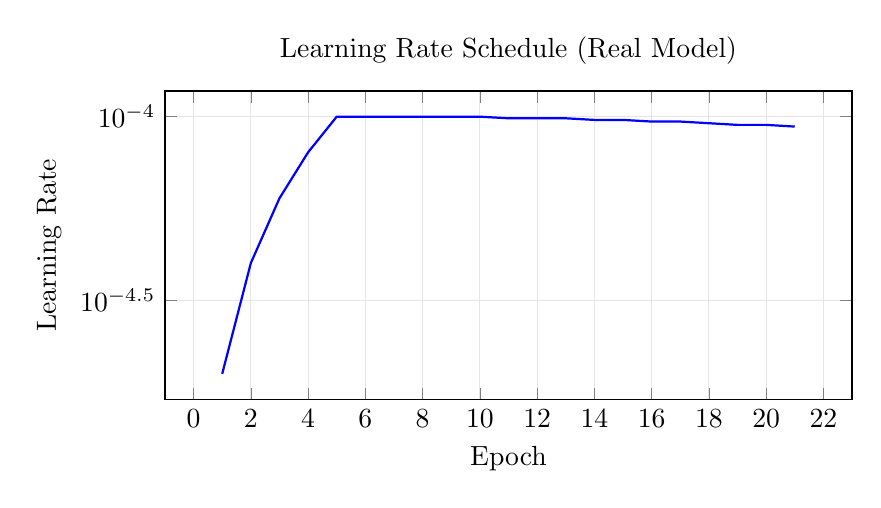
\begin{tikzpicture}
\begin{axis}[
    width=0.85\textwidth, height=5.5cm,
    xlabel={Epoch}, ylabel={Learning Rate},
    ymode=log,
    grid=both, grid style={gray!20},
    legend pos=north east,
    title={Learning Rate Schedule (Real Model)},
]
\addplot[blue, thick, mark=none] coordinates {
    (1,0.000020) (2,0.000040) (3,0.000060) (4,0.000080) (5,0.000100)
    (6,0.000100) (7,0.000100) (8,0.000100) (9,0.000100) (10,0.000100)
    (11,0.000099) (12,0.000099) (13,0.000099) (14,0.000098) (15,0.000098)
    (16,0.000097) (17,0.000097) (18,0.000096) (19,0.000095) (20,0.000095)
    (21,0.000094)
};
\end{axis}
\end{tikzpicture}
\caption{Learning rate schedule for the real-domain model showing linear warmup
(epochs 1--5) followed by cosine annealing decay.}
\label{fig:lr_schedule}
\end{figure}

\subsubsection{Mixup Augmentation}

Mixup~\cite{zhang2018mixup} is a data augmentation technique that creates
virtual training examples by linearly interpolating between pairs of training
samples and their labels:

\begin{equation}
\tilde{x} = \lambda x_i + (1 - \lambda) x_j, \qquad
\lambda \sim \text{Beta}(0.2, 0.2)
\end{equation}

\begin{equation}
\mathcal{L}_{\text{mixup}} = \lambda \cdot \text{CE}(\hat{y}, y_i) +
(1 - \lambda) \cdot \text{CE}(\hat{y}, y_j)
\end{equation}

The Beta(0.2, 0.2) distribution is U-shaped, meaning $\lambda$ tends to be
close to 0 or 1 so most mixed images look mostly like one of the two
originals, with a subtle blend of the other.  Mixup serves several purposes:
\begin{itemize}[leftmargin=*]
    \item \textbf{Regularisation:} It prevents the model from memorising
          individual training images, reducing overfitting.
    \item \textbf{Smoother decision boundaries:} The model learns to make
          gradual transitions between classes rather than sharp, brittle boundaries.
    \item \textbf{Improved cross-domain generalisation:} By training on
          interpolated images, the model is exposed to visual variations that
          are not present in the original dataset, helping it generalise to
          unseen domains.
\end{itemize}

Note that mixup causes training accuracy to appear lower than validation
accuracy this is expected, since the model is trained on blended images but
evaluated on clean ones.

\subsubsection{Loss Function: Weighted Cross-Entropy with Label Smoothing}

The loss function combines three mechanisms to handle the challenges of
multi-class classification with imbalanced data:

\begin{equation}
\mathcal{L} = \text{CrossEntropy}(\hat{y}, y; \mathbf{w}, \epsilon=0.1)
\end{equation}

\textbf{Cross-entropy loss} is the standard loss function for classification.
It measures the divergence between the predicted probability distribution and
the true label.  For a single sample with true class $c$:

\begin{equation}
\text{CE} = -\log \hat{p}_c
\end{equation}

where $\hat{p}_c$ is the model's predicted probability for the correct class.
The loss is zero when the model is perfectly confident in the correct class, and
increases as confidence drops.

\textbf{Class weighting} ($\mathbf{w}$) addresses class imbalance by
multiplying each sample's loss by its class weight $w_c$ from
Equation~\ref{eq:class_weights}.  Classes with fewer training samples receive
higher weights, so the model pays more attention to rare classes and does not
simply learn to always predict the majority class.  Without class weighting, a
model could achieve high overall accuracy by ignoring rare classes entirely.

\textbf{Label smoothing} ($\epsilon = 0.1$) replaces the hard one-hot target
$[0, 0, \ldots, 1, \ldots, 0]$ with a softened distribution:

\begin{equation}
y_{\text{smooth}}(k) =
\begin{cases}
1 - \epsilon + \epsilon / C & \text{if } k = c \\
\epsilon / C & \text{otherwise}
\end{cases}
\end{equation}

where $C = 81$ is the number of classes.  This prevents the model from becoming
\emph{overconfident} instead of driving logits to extreme values (which can
cause gradient saturation and poor calibration), it encourages the model to
maintain a small amount of uncertainty.  Label smoothing acts as a regulariser
and typically improves generalisation performance, especially under domain shift.

\subsubsection{Image Augmentation Pipeline}

The training transform chain applies aggressive augmentation to maximise
the model's exposure to visual variation:

\begin{enumerate}[leftmargin=*]
    \item \texttt{RandomResizedCrop}$(224, \text{scale}=(0.7, 1.0))$
    \item \texttt{RandomHorizontalFlip}
    \item \texttt{RandomRotation}$(\pm 15^{\circ})$
    \item \texttt{RandomAffine}$(\text{translate}=10\%, \text{scale}=(0.9, 1.1))$
    \item \texttt{ColorJitter}$(\text{brightness}=0.3, \text{contrast}=0.3,
          \text{saturation}=0.3, \text{hue}=0.1)$
    \item \texttt{RandomGrayscale}$(p=0.1)$
    \item \texttt{ToTensor} $\to$ \texttt{Normalize}(ImageNet mean/std)
    \item \texttt{RandomErasing}$(p=0.2)$
\end{enumerate}

Validation and test images use: \texttt{Resize}$(256) \to
\texttt{CenterCrop}(224) \to \texttt{ToTensor} \to \texttt{Normalize}$.

\subsubsection{Early Stopping and Checkpointing}

\begin{itemize}[leftmargin=*]
    \item Best model saved by \textbf{macro F1} on the validation set (rather
          than accuracy, because macro F1 equally weighs all classes regardless
          of support).
    \item Checkpoint saved every epoch to allow resumption after interruption.
    \item Early stopping triggers after $\texttt{patience} = 10$ epochs with no
          validation loss improvement, preventing wasted computation.
\end{itemize}

\subsection{Computational Resources}

Training was performed on an HPC cluster using SLURM:

\begin{table}[H]
\centering
\caption{SLURM resource allocation per training job.}
\label{tab:slurm}
\begin{tabular}{ll}
\toprule
\textbf{Resource} & \textbf{Allocation} \\
\midrule
Partition & H200 \\
Nodes     & 1 \\
CPUs      & 16 \\
GPUs      & 8 $\times$ NVIDIA H200 \\
Memory    & 200 GB \\
\bottomrule
\end{tabular}
\end{table}


% ══════════════════════════════════════════════════════════════════════════════
\section{Training Results}
\label{sec:training_results}

\subsection{Real-Domain Model}

The real-domain model was trained for 21 epochs before early stopping, with
convergence reaching a peak validation F1 (macro) of \textbf{0.9451} at epoch
9.

\begin{figure}[H]
\centering
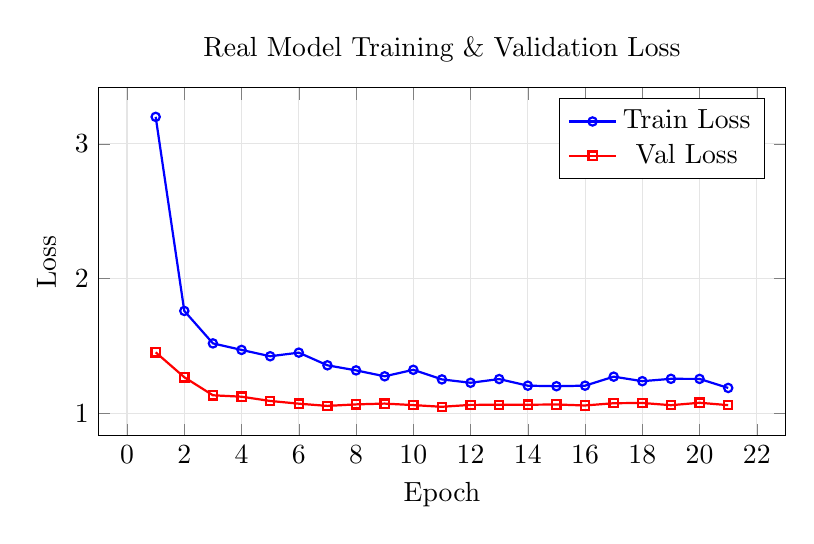
\begin{tikzpicture}
\begin{axis}[
    width=0.85\textwidth, height=6cm,
    xlabel={Epoch}, ylabel={Loss},
    grid=both, grid style={gray!20},
    legend pos=north east,
    title={Real Model Training \& Validation Loss},
]
\addplot[blue, thick, mark=o, mark size=1.5pt] coordinates {
    (1,3.2000) (2,1.7589) (3,1.5178) (4,1.4694) (5,1.4223)
    (6,1.4492) (7,1.3550) (8,1.3174) (9,1.2734) (10,1.3216)
    (11,1.2504) (12,1.2253) (13,1.2529) (14,1.2037) (15,1.1998)
    (16,1.2038) (17,1.2708) (18,1.2372) (19,1.2547) (20,1.2541)
    (21,1.1869)
};
\addlegendentry{Train Loss}
\addplot[red, thick, mark=square, mark size=1.5pt] coordinates {
    (1,1.4516) (2,1.2664) (3,1.1325) (4,1.1219) (5,1.0903)
    (6,1.0701) (7,1.0536) (8,1.0649) (9,1.0708) (10,1.0596)
    (11,1.0470) (12,1.0612) (13,1.0618) (14,1.0623) (15,1.0641)
    (16,1.0568) (17,1.0735) (18,1.0755) (19,1.0588) (20,1.0770)
    (21,1.0591)
};
\addlegendentry{Val Loss}
\end{axis}
\end{tikzpicture}
\caption{Training and validation loss curves for the real-domain model.  The
validation loss plateaus around epoch 11 ($\sim$1.047), triggering early
stopping at epoch 21.  Note that training loss is higher than validation loss
 this is expected with mixup augmentation.}
\label{fig:real_loss}
\end{figure}

\begin{figure}[H]
\centering
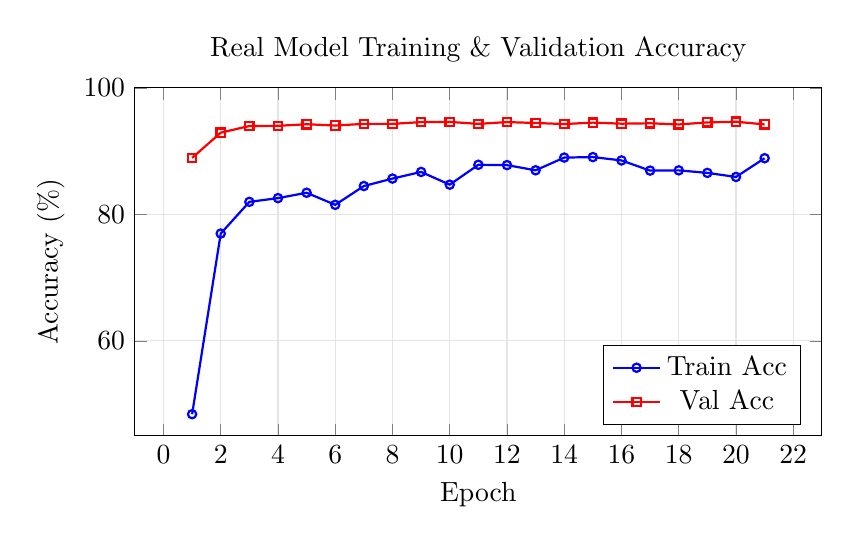
\begin{tikzpicture}
\begin{axis}[
    width=0.85\textwidth, height=6cm,
    xlabel={Epoch}, ylabel={Accuracy (\%)},
    grid=both, grid style={gray!20},
    legend pos=south east,
    title={Real Model Training \& Validation Accuracy},
    ymin=45, ymax=100,
]
\addplot[blue, thick, mark=o, mark size=1.5pt] coordinates {
    (1,48.41) (2,76.97) (3,81.98) (4,82.57) (5,83.42)
    (6,81.51) (7,84.48) (8,85.66) (9,86.71) (10,84.70)
    (11,87.84) (12,87.79) (13,86.97) (14,88.98) (15,89.06)
    (16,88.53) (17,86.92) (18,86.96) (19,86.56) (20,85.92)
    (21,88.88)
};
\addlegendentry{Train Acc}
\addplot[red, thick, mark=square, mark size=1.5pt] coordinates {
    (1,88.93) (2,92.92) (3,93.97) (4,94.00) (5,94.25)
    (6,94.05) (7,94.31) (8,94.31) (9,94.59) (10,94.62)
    (11,94.31) (12,94.59) (13,94.45) (14,94.28) (15,94.51)
    (16,94.34) (17,94.40) (18,94.22) (19,94.54) (20,94.65)
    (21,94.22)
};
\addlegendentry{Val Acc}
\end{axis}
\end{tikzpicture}
\caption{Training and validation accuracy for the real-domain model.  Validation
accuracy stabilises around 94.5\% from epoch 5 onward.}
\label{fig:real_acc}
\end{figure}

\begin{figure}[H]
\centering
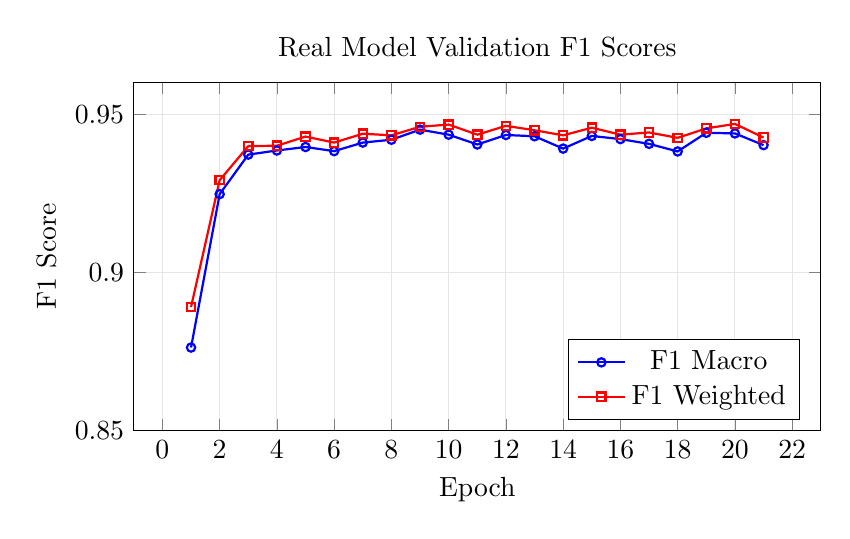
\begin{tikzpicture}
\begin{axis}[
    width=0.85\textwidth, height=6cm,
    xlabel={Epoch}, ylabel={F1 Score},
    grid=both, grid style={gray!20},
    legend pos=south east,
    title={Real Model  Validation F1 Scores},
    ymin=0.85, ymax=0.96,
]
\addplot[blue, thick, mark=o, mark size=1.5pt] coordinates {
    (1,0.8762) (2,0.9247) (3,0.9372) (4,0.9385) (5,0.9396)
    (6,0.9383) (7,0.9410) (8,0.9419) (9,0.9451) (10,0.9435)
    (11,0.9404) (12,0.9434) (13,0.9430) (14,0.9391) (15,0.9431)
    (16,0.9421) (17,0.9406) (18,0.9382) (19,0.9441) (20,0.9439)
    (21,0.9402)
};
\addlegendentry{F1 Macro}
\addplot[red, thick, mark=square, mark size=1.5pt] coordinates {
    (1,0.8890) (2,0.9291) (3,0.9399) (4,0.9400) (5,0.9429)
    (6,0.9410) (7,0.9438) (8,0.9433) (9,0.9460) (10,0.9467)
    (11,0.9435) (12,0.9463) (13,0.9449) (14,0.9433) (15,0.9457)
    (16,0.9435) (17,0.9442) (18,0.9425) (19,0.9455) (20,0.9469)
    (21,0.9426)
};
\addlegendentry{F1 Weighted}
\end{axis}
\end{tikzpicture}
\caption{Validation F1 scores for the real-domain model.  Both macro and
weighted F1 converge to $\sim$0.94.}
\label{fig:real_f1}
\end{figure}

\subsection{Sketch-Domain Model}

The sketch-domain model was trained for 19 epochs, achieving a peak validation
F1 (macro) of \textbf{0.8336} at epoch 13.

\begin{figure}[H]
\centering
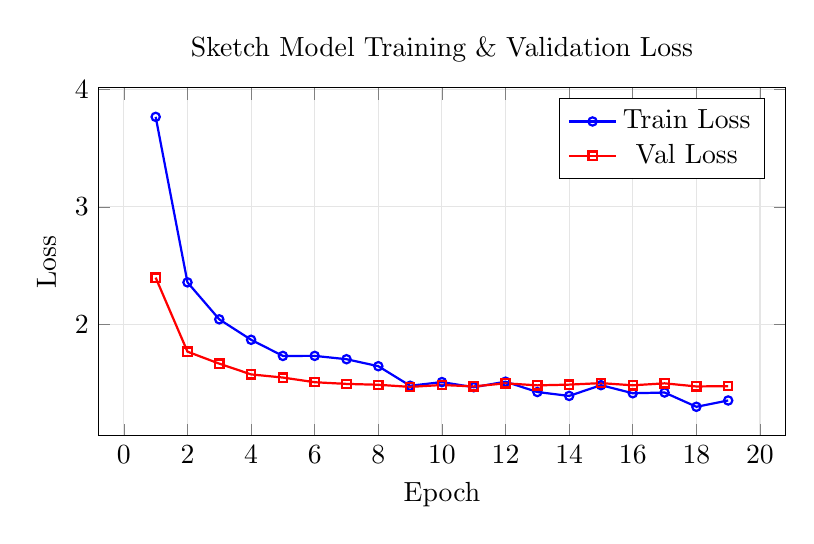
\begin{tikzpicture}
\begin{axis}[
    width=0.85\textwidth, height=6cm,
    xlabel={Epoch}, ylabel={Loss},
    grid=both, grid style={gray!20},
    legend pos=north east,
    title={Sketch Model Training \& Validation Loss},
]
\addplot[blue, thick, mark=o, mark size=1.5pt] coordinates {
    (1,3.7655) (2,2.3588) (3,2.0445) (4,1.8708) (5,1.7336)
    (6,1.7340) (7,1.7056) (8,1.6462) (9,1.4800) (10,1.5112)
    (11,1.4675) (12,1.5146) (13,1.4267) (14,1.3936) (15,1.4851)
    (16,1.4163) (17,1.4224) (18,1.3012) (19,1.3549)
};
\addlegendentry{Train Loss}
\addplot[red, thick, mark=square, mark size=1.5pt] coordinates {
    (1,2.3991) (2,1.7699) (3,1.6678) (4,1.5765) (5,1.5497)
    (6,1.5100) (7,1.4957) (8,1.4884) (9,1.4704) (10,1.4864)
    (11,1.4746) (12,1.5007) (13,1.4833) (14,1.4896) (15,1.5025)
    (16,1.4839) (17,1.5006) (18,1.4741) (19,1.4767)
};
\addlegendentry{Val Loss}
\end{axis}
\end{tikzpicture}
\caption{Training and validation loss curves for the sketch-domain model.
Convergence is slower and final loss is higher than the real model, reflecting
the greater challenge of learning from abstract sketches.}
\label{fig:sketch_loss}
\end{figure}

\begin{figure}[H]
\centering
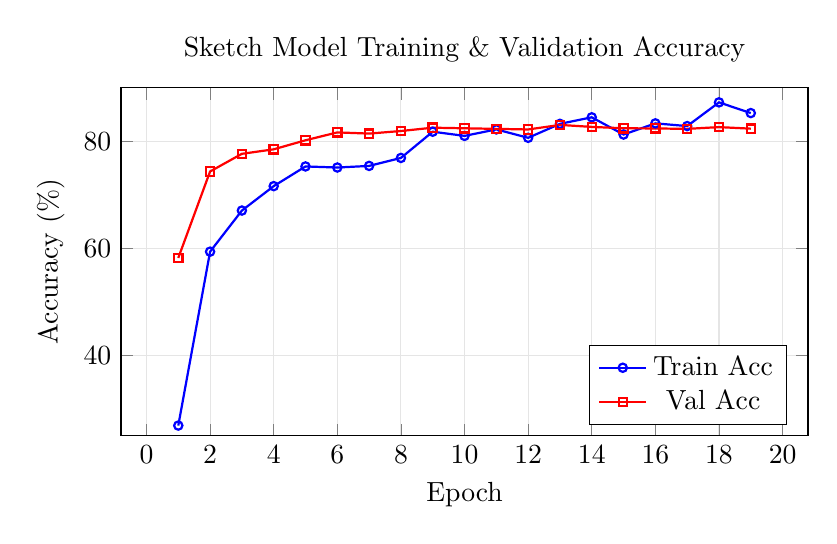
\begin{tikzpicture}
\begin{axis}[
    width=0.85\textwidth, height=6cm,
    xlabel={Epoch}, ylabel={Accuracy (\%)},
    grid=both, grid style={gray!20},
    legend pos=south east,
    title={Sketch Model  Training \& Validation Accuracy},
    ymin=25, ymax=90,
]
\addplot[blue, thick, mark=o, mark size=1.5pt] coordinates {
    (1,26.91) (2,59.40) (3,67.08) (4,71.64) (5,75.32)
    (6,75.12) (7,75.42) (8,76.91) (9,81.81) (10,81.03)
    (11,82.24) (12,80.67) (13,83.28) (14,84.50) (15,81.28)
    (16,83.37) (17,82.86) (18,87.29) (19,85.29)
};
\addlegendentry{Train Acc}
\addplot[red, thick, mark=square, mark size=1.5pt] coordinates {
    (1,58.22) (2,74.38) (3,77.68) (4,78.52) (5,80.21)
    (6,81.68) (7,81.46) (8,81.94) (9,82.56) (10,82.45)
    (11,82.34) (12,82.23) (13,83.08) (14,82.71) (15,82.45)
    (16,82.42) (17,82.34) (18,82.67) (19,82.38)
};
\addlegendentry{Val Acc}
\end{axis}
\end{tikzpicture}
\caption{Training and validation accuracy for the sketch-domain model.
Validation accuracy plateaus around 82--83\%.}
\label{fig:sketch_acc}
\end{figure}

\begin{figure}[H]
\centering
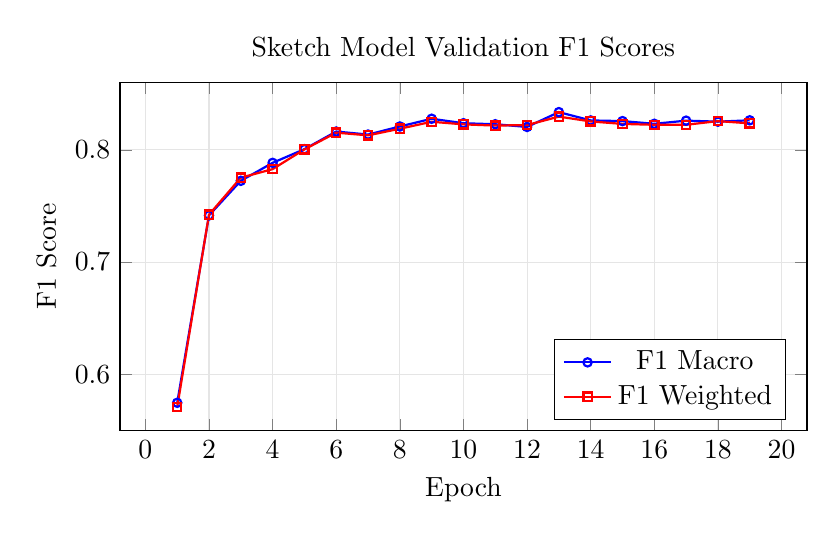
\begin{tikzpicture}
\begin{axis}[
    width=0.85\textwidth, height=6cm,
    xlabel={Epoch}, ylabel={F1 Score},
    grid=both, grid style={gray!20},
    legend pos=south east,
    title={Sketch Model Validation F1 Scores},
    ymin=0.55, ymax=0.86,
]
\addplot[blue, thick, mark=o, mark size=1.5pt] coordinates {
    (1,0.5746) (2,0.7416) (3,0.7724) (4,0.7884) (5,0.8006)
    (6,0.8163) (7,0.8136) (8,0.8208) (9,0.8277) (10,0.8237)
    (11,0.8228) (12,0.8204) (13,0.8336) (14,0.8262) (15,0.8256)
    (16,0.8232) (17,0.8260) (18,0.8251) (19,0.8263)
};
\addlegendentry{F1 Macro}
\addplot[red, thick, mark=square, mark size=1.5pt] coordinates {
    (1,0.5709) (2,0.7422) (3,0.7752) (4,0.7828) (5,0.8004)
    (6,0.8153) (7,0.8129) (8,0.8188) (9,0.8250) (10,0.8227)
    (11,0.8216) (12,0.8221) (13,0.8296) (14,0.8253) (15,0.8231)
    (16,0.8223) (17,0.8223) (18,0.8256) (19,0.8236)
};
\addlegendentry{F1 Weighted}
\end{axis}
\end{tikzpicture}
\caption{Validation F1 scores for the sketch-domain model.}
\label{fig:sketch_f1}
\end{figure}

\subsection{Precision and Recall Curves}

\begin{figure}[H]
\centering
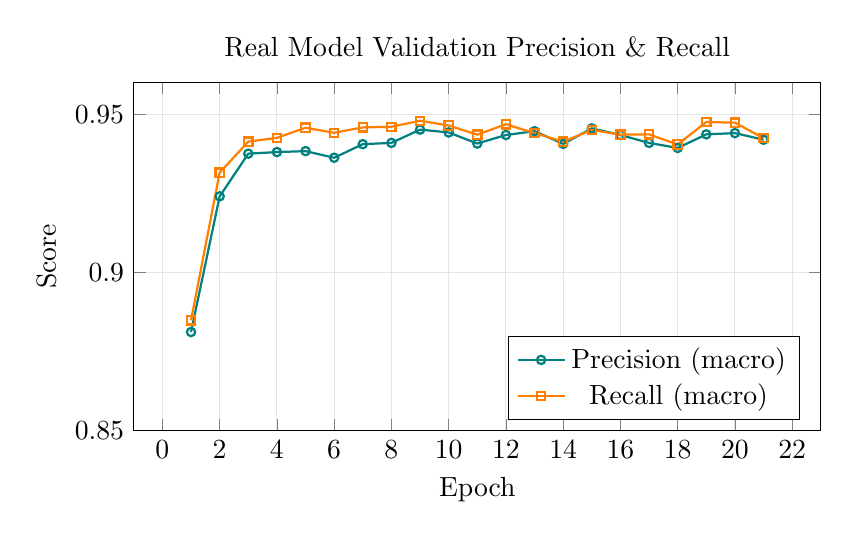
\begin{tikzpicture}
\begin{axis}[
    width=0.85\textwidth, height=6cm,
    xlabel={Epoch}, ylabel={Score},
    grid=both, grid style={gray!20},
    legend pos=south east,
    title={Real Model Validation Precision \& Recall},
    ymin=0.85, ymax=0.96,
]
\addplot[teal, thick, mark=o, mark size=1.5pt] coordinates {
    (1,0.8811) (2,0.9240) (3,0.9375) (4,0.9380) (5,0.9383)
    (6,0.9362) (7,0.9405) (8,0.9409) (9,0.9451) (10,0.9442)
    (11,0.9407) (12,0.9434) (13,0.9446) (14,0.9406) (15,0.9455)
    (16,0.9434) (17,0.9409) (18,0.9393) (19,0.9436) (20,0.9440)
    (21,0.9419)
};
\addlegendentry{Precision (macro)}
\addplot[orange, thick, mark=square, mark size=1.5pt] coordinates {
    (1,0.8848) (2,0.9315) (3,0.9413) (4,0.9425) (5,0.9457)
    (6,0.9441) (7,0.9458) (8,0.9460) (9,0.9479) (10,0.9464)
    (11,0.9435) (12,0.9468) (13,0.9440) (14,0.9413) (15,0.9450)
    (16,0.9435) (17,0.9436) (18,0.9404) (19,0.9475) (20,0.9473)
    (21,0.9424)
};
\addlegendentry{Recall (macro)}
\end{axis}
\end{tikzpicture}
\caption{Validation precision and recall for the real-domain model.}
\label{fig:real_prec_recall}
\end{figure}

\begin{figure}[H]
\centering
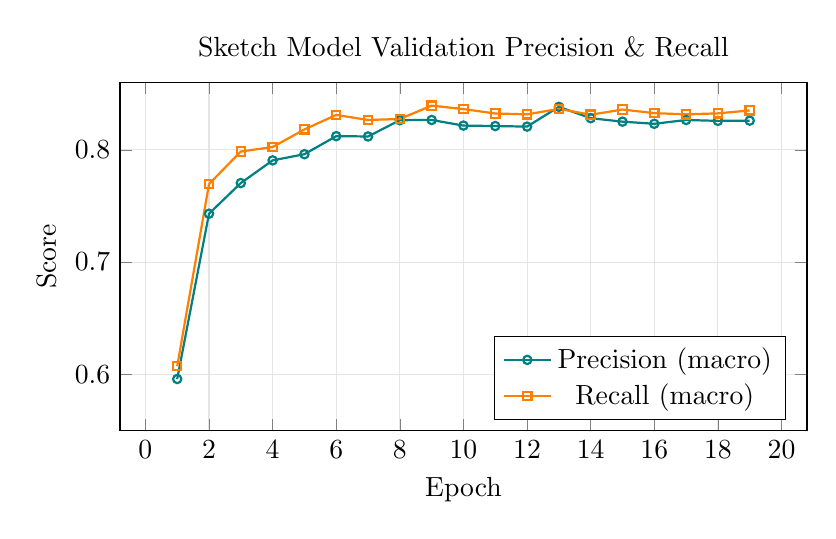
\begin{tikzpicture}
\begin{axis}[
    width=0.85\textwidth, height=6cm,
    xlabel={Epoch}, ylabel={Score},
    grid=both, grid style={gray!20},
    legend pos=south east,
    title={Sketch Model Validation Precision \& Recall},
    ymin=0.55, ymax=0.86,
]
\addplot[teal, thick, mark=o, mark size=1.5pt] coordinates {
    (1,0.5958) (2,0.7431) (3,0.7704) (4,0.7906) (5,0.7961)
    (6,0.8122) (7,0.8119) (8,0.8264) (9,0.8266) (10,0.8216)
    (11,0.8212) (12,0.8207) (13,0.8383) (14,0.8282) (15,0.8251)
    (16,0.8232) (17,0.8266) (18,0.8258) (19,0.8260)
};
\addlegendentry{Precision (macro)}
\addplot[orange, thick, mark=square, mark size=1.5pt] coordinates {
    (1,0.6072) (2,0.7695) (3,0.7985) (4,0.8025) (5,0.8182)
    (6,0.8311) (7,0.8266) (8,0.8275) (9,0.8394) (10,0.8363)
    (11,0.8324) (12,0.8316) (13,0.8365) (14,0.8313) (15,0.8359)
    (16,0.8327) (17,0.8316) (18,0.8325) (19,0.8351)
};
\addlegendentry{Recall (macro)}
\end{axis}
\end{tikzpicture}
\caption{Validation precision and recall for the sketch-domain model.}
\label{fig:sketch_prec_recall}
\end{figure}


% ══════════════════════════════════════════════════════════════════════════════
\section{Evaluation Results}
\label{sec:evaluation}

Each trained model is evaluated on both the in-domain and cross-domain test
sets.  This produces four evaluation scenarios.

\subsection{Overall Metrics}

\begin{table}[H]
\centering
\caption{Classification performance across all evaluation scenarios.  Bold
values indicate the best score in each column.}
\label{tab:eval_metrics}
\begin{tabular}{llccccc}
\toprule
\textbf{Train} & \textbf{Test} & \textbf{Accuracy} & \textbf{F1 Macro}
& \textbf{F1 Weighted} & \textbf{Precision} & \textbf{Recall} \\
\midrule
Real   & Real   & \textbf{93.63\%} & \textbf{0.9288} & \textbf{0.9365}
       & 0.9276 & \textbf{0.9334} \\
Real   & Sketch & 56.17\%          & 0.5695          & 0.5837
       & 0.6804 & 0.5755 \\
Sketch & Sketch & 80.62\%          & 0.8087          & 0.8057
       & 0.8103 & 0.8178 \\
Sketch & Real   & 83.02\%          & 0.8164          & 0.8313
       & \textbf{0.8425} & 0.8193 \\
\bottomrule
\end{tabular}
\end{table}

\subsection{Key Observations}

\begin{enumerate}[leftmargin=*]
    \item \textbf{Real model in-domain:} Achieves the highest accuracy
          (93.63\%) and F1 (0.9288), benefiting from the rich texture and
          colour information in photographs.
    \item \textbf{Sketch model in-domain:} Achieves 80.62\% accuracy.  Sketches
          are inherently more variable and abstract, making classification
          harder.
    \item \textbf{Asymmetric transfer:} The sketch-trained model transfers
          remarkably well to real images (83.02\%), outperforming the
          real-trained model on sketches (56.17\%) by a wide margin.  This
          suggests that sketch training forces the model to learn
          \emph{structural} features (shape, contour, spatial layout) that
          generalise across domains, while real training encourages reliance on
          \emph{texture} features that do not transfer to sketches.
    \item \textbf{Texture bias:} The real$\to$sketch drop of 37.46 percentage
          points is consistent with the known texture bias of CNNs trained on
          photographs~\cite{geirhos2019texture}.
\end{enumerate}

\subsection{Cross-Domain Transfer Comparison}

\begin{figure}[H]
\centering
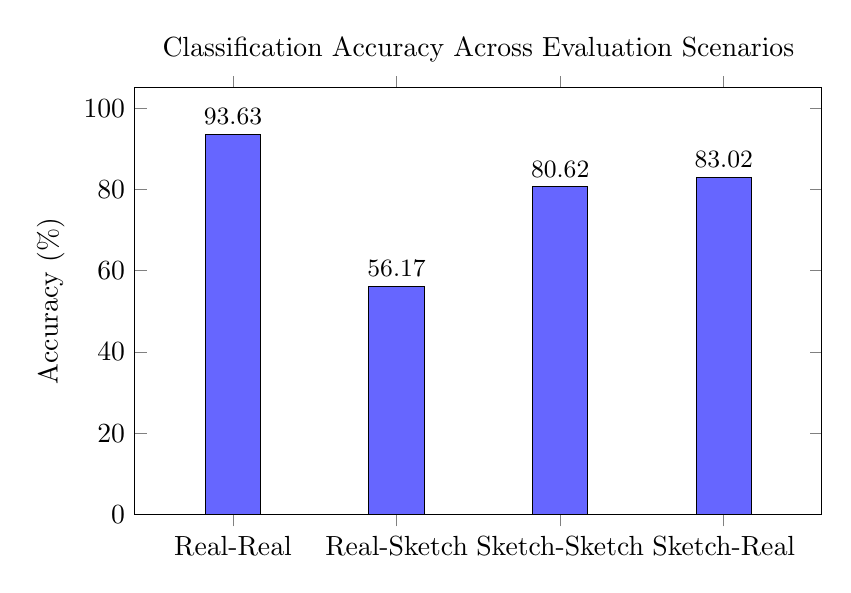
\begin{tikzpicture}
\begin{axis}[
    ybar,
    width=0.85\textwidth, height=7cm,
    ylabel={Accuracy (\%)},
    symbolic x coords={Real-Real, Real-Sketch, Sketch-Sketch, Sketch-Real},
    xtick=data,
    nodes near coords,
    nodes near coords align={vertical},
    every node near coord/.append style={font=\small},
    ymin=0, ymax=105,
    bar width=20pt,
    title={Classification Accuracy Across Evaluation Scenarios},
    enlarge x limits=0.2,
]
\addplot[fill=blue!60] coordinates {
    (Real-Real, 93.63) (Real-Sketch, 56.17)
    (Sketch-Sketch, 80.62) (Sketch-Real, 83.02)
};
\end{axis}
\end{tikzpicture}
\caption{Classification accuracy across all four evaluation scenarios.  The
sketch$\to$real transfer (83.02\%) substantially outperforms real$\to$sketch
(56.17\%).}
\label{fig:eval_bar}
\end{figure}

\begin{figure}[H]
\centering
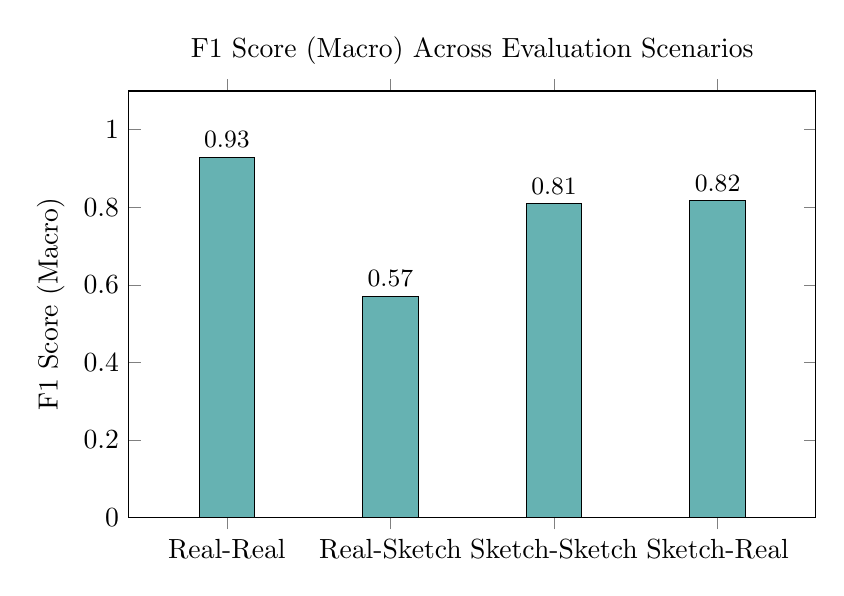
\begin{tikzpicture}
\begin{axis}[
    ybar,
    width=0.85\textwidth, height=7cm,
    ylabel={F1 Score (Macro)},
    symbolic x coords={Real-Real, Real-Sketch, Sketch-Sketch, Sketch-Real},
    xtick=data,
    nodes near coords,
    nodes near coords align={vertical},
    every node near coord/.append style={font=\small},
    ymin=0, ymax=1.1,
    bar width=20pt,
    title={F1 Score (Macro) Across Evaluation Scenarios},
    enlarge x limits=0.2,
]
\addplot[fill=teal!60] coordinates {
    (Real-Real, 0.9288) (Real-Sketch, 0.5695)
    (Sketch-Sketch, 0.8087) (Sketch-Real, 0.8164)
};
\end{axis}
\end{tikzpicture}
\caption{Macro F1 scores across evaluation scenarios.}
\label{fig:eval_f1_bar}
\end{figure}

\subsection{Confusion Matrix Analysis}

Confusion matrices were generated for all four evaluation scenarios.  Each
matrix covers all 81 classes with balanced sampling (9 images per class) for
fair comparison.

\begin{figure}[H]
\centering

\includegraphics[width=0.95\textwidth]{output/evaluation/real_model_on_real/confusion_matrix.png}
\caption{Confusion matrix for the real model evaluated on the real test set
(in-domain).  The strong diagonal indicates high classification accuracy
across most classes.}
\label{fig:cm_real_real}
\end{figure}

\begin{figure}[H]
\centering

\includegraphics[width=0.95\textwidth]{output/evaluation/real_model_on_sketch/confusion_matrix.png}
\caption{Confusion matrix for the real model evaluated on the sketch test set
(cross-domain).  Significant off-diagonal activity reveals systematic
cross-domain confusion patterns.}
\label{fig:cm_real_sketch}
\end{figure}

\begin{figure}[H]
\centering

\includegraphics[width=0.95\textwidth]{output/evaluation/sketch_model_on_sketch/confusion_matrix.png}
\caption{Confusion matrix for the sketch model evaluated on the sketch test set
(in-domain).}
\label{fig:cm_sketch_sketch}
\end{figure}

\begin{figure}[H]
\centering

\includegraphics[width=0.95\textwidth]{output/evaluation/sketch_model_on_real/confusion_matrix.png}
\caption{Confusion matrix for the sketch model evaluated on the real test set
(cross-domain).  Despite the domain shift, classification remains surprisingly
accurate.}
\label{fig:cm_sketch_real}
\end{figure}

\subsection{Training Summaries}

\begin{figure}[H]
\centering

\includegraphics[width=0.85\textwidth]{output/evaluation/real_model_on_real/training_summary.png}
\caption{Combined training summary for the real-domain model (2$\times$2 grid:
loss, accuracy, F1, precision/recall).}
\label{fig:real_training_summary}
\end{figure}

\begin{figure}[H]
\centering

\includegraphics[width=0.85\textwidth]{output/evaluation/sketch_model_on_sketch/training_summary.png}
\caption{Combined training summary for the sketch-domain model.}
\label{fig:sketch_training_summary}
\end{figure}

\subsection{Top and Bottom Performing Classes}

\subsubsection{Real Model (In-Domain: Real $\to$ Real)}

\begin{table}[H]
\centering
\caption{Top 10 and bottom 10 classes by accuracy for the real model evaluated
on the real test set.}
\label{tab:top_bottom_real}
\begin{tabular}{lrr|lrr}
\toprule
\multicolumn{3}{c|}{\textbf{Top 10}} & \multicolumn{3}{c}{\textbf{Bottom 10}} \\
\textbf{Class} & \textbf{Acc\%} & \textbf{F1} &
\textbf{Class} & \textbf{Acc\%} & \textbf{F1} \\
\midrule
The Mona Lisa     & 100.0 & 0.983 & saw        & 66.67 & 0.696 \\
basketball        & 100.0 & 1.000 & eye        & 75.36 & 0.846 \\
saxophone         & 100.0 & 1.000 & circle     & 80.77 & 0.857 \\
skull              & 100.0 & 1.000 & spoon      & 81.13 & 0.878 \\
trumpet           & 100.0 & 1.000 & triangle   & 81.58 & 0.838 \\
backpack          & 100.0 & 0.936 & flower     & 83.33 & 0.896 \\
banana            & 100.0 & 0.963 & barn       & 83.87 & 0.881 \\
baseball          & 100.0 & 0.900 & shovel     & 84.44 & 0.905 \\
firetruck         & 100.0 & 0.974 & feather    & 86.00 & 0.860 \\
spreadsheet       & 100.0 & 0.987 & suitcase   & 86.05 & 0.914 \\
\bottomrule
\end{tabular}
\end{table}

\textbf{Analysis:} The real model excels at classes with highly distinctive
visual features: \emph{saxophone} has a unique metallic curved shape,
\emph{ladder} has a distinctive A-frame structure with repeating rungs, and \emph{trumpet}
has a distinctive bell shape.  The bottom performers reveal interesting failure
patterns: \emph{saw} (66.67\%) is often confused with other elongated tools;
\emph{circle} and \emph{triangle} lack the rich texture cues that the
real model relies on; and \emph{spoon} shares visual similarity with other
utensils.

\subsubsection{Sketch Model (In-Domain: Sketch $\to$ Sketch)}

\begin{table}[H]
\centering
\caption{Top 10 and bottom 10 classes by accuracy for the sketch model
evaluated on the sketch test set.}
\label{tab:top_bottom_sketch}
\begin{tabular}{lrr|lrr}
\toprule
\multicolumn{3}{c|}{\textbf{Top 10}} & \multicolumn{3}{c}{\textbf{Bottom 10}} \\
\textbf{Class} & \textbf{Acc\%} & \textbf{F1} &
\textbf{Class} & \textbf{Acc\%} & \textbf{F1} \\
\midrule
banana       & 100.0 & 0.952 & shovel     & 44.44 & 0.544 \\
barn         & 100.0 & 0.930 & scorpion   & 55.56 & 0.694 \\
baseball     & 100.0 & 0.833 & sword      & 55.26 & 0.568 \\
bicycle      & 100.0 & 1.000 & firetruck  & 57.58 & 0.623 \\
marker       & 100.0 & 0.828 & triangle   & 60.00 & 0.667 \\
axe          & 95.45 & 0.840 & saw        & 63.64 & 0.667 \\
birthday cake & 95.65 & 0.936 & palm tree  & 64.71 & 0.550 \\
light bulb   & 95.00 & 0.905 & sock       & 64.44 & 0.699 \\
tiger        & 94.87 & 0.925 & circle     & 65.00 & 0.578 \\
laptop       & 93.75 & 0.896 & scissors   & 65.91 & 0.674 \\
\bottomrule
\end{tabular}
\end{table}

\textbf{Analysis:} The sketch model's top performers include classes with
structurally distinctive shapes that are easy to draw consistently:
\emph{bicycle} has its iconic two-wheel-and-frame structure, \emph{banana} has
a unique curved shape, and \emph{barn} has a recognisable rooftop silhouette.
The bottom performers reveal that sketch classification is hardest for
\emph{elongated tools} (shovel at 44.44\%, sword at 55.26\%, saw at 63.64\%)
whose sketches look similar, and \emph{simple geometric shapes} (triangle at
60.00\%, circle at 65.00\%) that lack distinguishing internal detail.
Interestingly, \emph{firetruck} drops from 100\% in the real model to 57.58\%
in the sketch model likely because sketches of firetrucks lack the
distinctive red colour and detailed ladder/hose features that make them easy
to identify in photographs.


% ══════════════════════════════════════════════════════════════════════════════
\section{XAI Methods}
\label{sec:xai_methods}

Deep neural networks achieve impressive accuracy, but they function as
``black boxes'' they do not explain \emph{why} they make a particular
prediction.  \textbf{Attribution methods} (also called \emph{saliency methods})
address this by assigning an importance score to every spatial location in the
input image.  The result is a \textbf{heatmap} that highlights the pixels or
regions that were most influential to the model's decision.  For example, if
the model predicts ``ladder'', the heatmap should highlight the rungs and
rails rather than the background.

In this project we apply four complementary attribution methods.  Each takes a
different approach to the same question:
\textit{``Which pixels drove the model to predict this class?''}
Understanding the differences between these methods is essential for
interpreting the results that follow.


% ────────────────────────────────────────────────────────────────────────
\subsection{Method 1: Grad-CAM}

\textbf{Gradient-weighted Class Activation Mapping}~\cite{selvaraju2017gradcam}
is one of the most widely used XAI methods in computer vision.  It works by
looking at the \emph{last convolutional layer} of the network the layer
that still retains spatial information (i.e., it knows \emph{where} things are
in the image) while also encoding high-level semantic concepts (i.e., it knows
\emph{what} things look like).

\subsubsection{Background: Why the Last Convolutional Layer?}

A convolutional neural network (CNN) like ResNet-152 processes an image through
a series of layers that progressively extract more abstract features:
\begin{itemize}[leftmargin=*]
    \item \textbf{Early layers} (conv1, layer1) detect simple patterns 
          edges, corners, colour gradients.
    \item \textbf{Middle layers} (layer2, layer3) combine these into textures,
          parts, and object fragments.
    \item \textbf{Late layers} (layer4) detect high-level concepts ``this
          region contains a wheel'', ``this region has a face''.
\end{itemize}

After the last convolutional layer (\texttt{layer4}), the spatial information
is collapsed into a single vector by global average pooling, and a fully
connected layer produces class scores.  Grad-CAM taps into the network
\emph{just before} this collapse, capturing both \emph{what} the model has
learned and \emph{where} in the image each concept appears.

\subsubsection{Step-by-Step Computation}

\begin{enumerate}[leftmargin=*]
    \item \textbf{Forward pass:} The input image ($224 \times 224 \times 3$) is
          fed through the network.  Using a PyTorch \emph{forward hook} on
          \texttt{layer4}, we record the output \textbf{feature maps}
          $\mathbf{A} \in \mathbb{R}^{2048 \times 7 \times 7}$.  Think of
          this as 2{,}048 small $7 \times 7$ images, each encoding a different
          visual pattern.  For example, one channel might activate strongly
          wherever it sees ``fur texture'', another where it sees ``circular
          shape'', etc.

    \item \textbf{Backward pass:} We select the class we want to explain (say,
          ``ladder'') and compute the gradient of its score $y^c$ with
          respect to the feature maps:
          $\frac{\partial y^c}{\partial \mathbf{A}}$.  These gradients tell us
          how a small change at each spatial location in each feature channel
          would affect the ladder score.  Channels and locations with large
          positive gradients are ``helpful'' for predicting ladder.

    \item \textbf{Global average pooling of gradients:} We average each
          channel's gradients over its $7 \times 7$ spatial grid to get a
          single importance weight per channel:
          \begin{equation}
          \alpha_k = \frac{1}{Z} \sum_{i,j} \frac{\partial y^c}{\partial A_{k,i,j}}
          \end{equation}
          A high $\alpha_k$ means that channel $k$'s feature pattern is
          important for class $c$.  For example, if the ``wheel'' channel has
          a high weight for ``bicycle'', it means the model considers wheels
          to be strong evidence for bicycles.

    \item \textbf{Weighted combination + ReLU:} We multiply each feature map
          by its importance weight and sum:
          \begin{equation}
          L_{\text{Grad-CAM}} = \text{ReLU}\left(\sum_k \alpha_k A_k\right)
          \end{equation}
          The ReLU (Rectified Linear Unit) clips negative values to zero.
          This is important: negative values correspond to features that
          belong to \emph{other} classes, not the one we are explaining.
          For example, if we ask ``why ladder?'', we do not want the
          heatmap to highlight regions that look like ``bicycle''.

    \item \textbf{Upsampling:} The resulting $7 \times 7$ heatmap is bilinearly
          interpolated to $224 \times 224$ pixels so it can be overlaid on the
          original image.
\end{enumerate}

\subsubsection{Strengths and Limitations}

\textbf{Strengths:}
\begin{itemize}[leftmargin=*]
    \item \textbf{Fast:} Only one forward pass and one backward pass required.
    \item \textbf{Class-discriminative:} Asking about different classes produces
          different heatmaps, so we can see what the model focuses on for each
          class.
    \item \textbf{Intuitive:} The output is a smooth, easily interpretable
          heatmap.
\end{itemize}

\textbf{Limitations:}
\begin{itemize}[leftmargin=*]
    \item \textbf{Coarse resolution:} The base heatmap is only $7 \times 7$.
          It shows \emph{which region} matters but not \emph{which specific
          pixels} within that region.  Fine details (e.g., individual stripes
          on a tiger) are lost.
    \item \textbf{Single-instance bias:} When multiple objects of the same
          class appear, Grad-CAM tends to highlight only the most prominent
          one.
    \item \textbf{No formal guarantees:} The method is a heuristic there
          is no mathematical proof that the highlighted region is truly
          ``the reason'' for the prediction.
\end{itemize}


% ────────────────────────────────────────────────────────────────────────
\subsection{Method 2: Grad-CAM++}

\textbf{Grad-CAM++}~\cite{chattopadhay2018gradcampp} is a refined version of
Grad-CAM that addresses two practical problems: (1)~Grad-CAM often highlights
only the most discriminative part of an object (e.g., the face of a dog but not
the body), and (2)~it struggles when multiple instances of the same class appear
in the image (e.g., a flock of birds).

\subsubsection{The Core Improvement}

The only change from Grad-CAM is \emph{how the channel importance weights are
computed}.  Instead of simple global average pooling of gradients, Grad-CAM++
uses \textbf{higher-order derivatives} (second and third derivatives of the
class score) to compute pixel-wise importance weights:

\begin{equation}
\alpha_k^c = \sum_{i,j} \underbrace{\frac{\left(\frac{\partial^2 y^c}{\partial A_k^2}\right)}
{2 \left(\frac{\partial^2 y^c}{\partial A_k^2}\right) +
\sum_{a,b} A_k \left(\frac{\partial^3 y^c}{\partial A_k^3}\right) + \epsilon}}_{\text{pixel-wise weight } w_{k,i,j}}
\end{equation}

\subsubsection{Intuition Behind the Formula}

Imagine you are trying to decide how important each region of a feature map is
for predicting ``dog''.  Grad-CAM asks: ``On average across all positions, does
this channel help predict dog?''  Grad-CAM++ asks a more refined question:
``\emph{At each specific position}, how much does this pixel contribute to the
positive evidence for dog?''

By considering second-order derivatives ($\partial^2 y^c / \partial A_k^2$),
the method captures \emph{curvature} information not just whether the
gradient is positive, but how quickly it is changing.  The third-order term
provides additional correction for numerical stability.

The practical effect is that Grad-CAM++ distributes attention more evenly
across the entire object:
\begin{itemize}[leftmargin=*]
    \item Grad-CAM on a dog might highlight only the face.
    \item Grad-CAM++ on the same dog will highlight the face, body, legs, and
          tail capturing the \emph{full extent} of the object.
\end{itemize}

\subsubsection{Strengths and Limitations}

\textbf{Strengths:}
\begin{itemize}[leftmargin=*]
    \item Better \emph{full object coverage} the heatmap covers more of the
          relevant region, not just the single most discriminative part.
    \item More numerically stable weights due to the higher-order formulation.
    \item Better multi-instance localisation when several objects of the same
          class appear in the image.
    \item Same computational cost as Grad-CAM (one forward + backward pass).
\end{itemize}

\textbf{Limitations:}
\begin{itemize}[leftmargin=*]
    \item Still limited to $7 \times 7$ spatial resolution (same upsampling
          trade-off as Grad-CAM).
    \item The higher-order gradient computation can be unstable for some
          architectures (though it works well for ResNets).
    \item Still a heuristic without formal axiomatic guarantees.
\end{itemize}


% ────────────────────────────────────────────────────────────────────────
\subsection{Method 3: Integrated Gradients}

\textbf{Integrated Gradients} (IG)~\cite{sundararajan2017ig} takes a
fundamentally different approach from the CAM-based methods.  Instead of
looking at intermediate feature maps, IG computes attributions directly at the
\textbf{input pixel level}, producing a $224 \times 224$ resolution attribution
map.  It is the \emph{only} method in our study that comes with formal
mathematical guarantees.

\subsubsection{The Problem with Simple Gradients}

One might think: ``Why not just compute the gradient of the class score with
respect to each input pixel?  Large gradients mean important pixels.''  This
is called the \emph{vanilla gradient} approach, and it has a critical flaw:
\textbf{gradient saturation}.  Neural networks with ReLU activations have
\emph{flat} regions where the gradient is zero even though the feature is
important.  A pixel might be crucial for the prediction, but if the network is
already saturated at that point, the gradient is zero and the pixel gets no
attribution.

Integrated Gradients solves this by integrating gradients along a \emph{path}
from a baseline to the input, ensuring every important feature receives credit.

\subsubsection{Axiomatic Foundation}

IG is designed to satisfy two formal axioms that any ``fair'' attribution method
should obey:

\begin{itemize}[leftmargin=*]
    \item \textbf{Sensitivity:} If changing a single feature (pixel) changes
          the model's output, that feature \emph{must} receive a non-zero
          attribution.  This prevents the ``blind spot'' problem of vanilla
          gradients.
    \item \textbf{Completeness:} The sum of all pixel attributions must
          \emph{exactly equal} the difference between the model's output for
          the input and the baseline:
          \begin{equation}
          \sum_i \text{IG}_i(x) = F(x) - F(x')
          \end{equation}
          This means attributions are \emph{additive} and
          \emph{budget-balanced} no importance is lost or fabricated.
\end{itemize}

\subsubsection{Step-by-Step Computation}

\begin{enumerate}[leftmargin=*]
    \item \textbf{Choose a baseline} $x'$:  The baseline represents ``absence
          of information''.  We use a \textbf{black image} (zero tensor after
          ImageNet normalisation).  The idea is: \emph{``What would the model
          see if nothing were present?''}  The difference between what the
          model predicts for a blank image vs.\ the actual image is what we
          want to attribute.

    \item \textbf{Create interpolated images:}  We create $n = 100$
          intermediate images that gradually blend from the baseline to the
          actual input:
          \[
          x_\alpha = x' + \alpha(x - x') \quad
          \text{for } \alpha = 0, \tfrac{1}{100}, \tfrac{2}{100}, \ldots, 1
          \]
          Imagine slowly ``fading in'' the photograph from black.  At
          $\alpha = 0$ we have the blank baseline; at $\alpha = 1$ we have
          the full image.

    \item \textbf{Compute gradients at each step:}  For each interpolated
          image, we compute the gradient of the class score with respect to
          the input pixels.  This tells us, at each point along the fade-in
          path, which pixels are currently contributing most.

    \item \textbf{Integrate the gradients:}  We average (numerically integrate
          using the trapezoidal rule) all these gradients and multiply by the
          pixel difference $(x - x')$:
          \begin{equation}
          \text{IG}_i(x) = (x_i - x_i') \times \int_0^1
          \frac{\partial F(x' + \alpha(x - x'))}{\partial x_i} \, d\alpha
          \end{equation}

    \item \textbf{Aggregate across colour channels:}  The attribution is
          computed for each of the 3 RGB channels independently; we take the
          absolute value and sum across channels to get a single per-pixel
          importance score.
\end{enumerate}

\subsubsection{Intuition: Why Integration Helps}

Consider a pixel that is vital for recognising a tiger's stripe.  At the
baseline (black image), this pixel contributes nothing.  As we fade the image
in, there is a critical moment when this pixel ``activates'' the stripe
detector in the network the gradient spikes at that moment.  By integrating
over the entire path, IG captures this spike even if the gradient is zero at
the endpoints.  Simple gradient methods would miss it entirely.

\subsubsection{Strengths and Limitations}

\textbf{Strengths:}
\begin{itemize}[leftmargin=*]
    \item \textbf{Pixel-level resolution} ($224 \times 224$) reveals fine
          details like individual stripes, edges, or small distinguishing
          features.
    \item \textbf{Mathematically principled} the axioms guarantee
          completeness and sensitivity.
    \item \textbf{Architecture-agnostic} works for any differentiable
          model (CNNs, transformers, etc.).
\end{itemize}

\textbf{Limitations:}
\begin{itemize}[leftmargin=*]
    \item \textbf{Slow:} Requires $n + 1 = 101$ forward and backward passes
          per image ($\sim$100$\times$ slower than Grad-CAM).
    \item \textbf{Noisier heatmaps:} Because it operates at full pixel
          resolution with no spatial smoothing, the output can appear noisy
          and harder to interpret visually.
    \item \textbf{Baseline-dependent:} The choice of baseline (black, white,
          random noise) can influence the attributions.
\end{itemize}


% ────────────────────────────────────────────────────────────────────────
\subsection{Method 4: LIME}

\textbf{Local Interpretable Model-agnostic Explanations}~\cite{ribeiro2016lime}
takes a fundamentally different philosophy: it does not look inside the network
at all.  Instead, it treats the neural network as a complete \textbf{black box}
and explains predictions by observing how the model's output changes when parts
of the input are hidden.

\subsubsection{The Core Idea}

Imagine covering parts of a photograph with grey patches and seeing how the
model's prediction changes.  If covering the dog's face causes the ``dog''
probability to drop sharply, the face is clearly important.  LIME automates
this process by:
\begin{enumerate}[leftmargin=*]
    \item Dividing the image into meaningful \emph{regions} (superpixels).
    \item Systematically hiding different combinations of regions.
    \item Fitting a simple model (linear regression) to learn which regions
          matter most.
\end{enumerate}

\subsubsection{Step-by-Step Computation}

\begin{enumerate}[leftmargin=*]
    \item \textbf{Segment the image into superpixels:}  Using the quickshift
          segmentation algorithm, the image is divided into $\sim$150
          superpixels contiguous regions of visually similar pixels.  Each
          superpixel might correspond to a patch of sky, a section of a
          wheel, or part of a face.

    \item \textbf{Generate 3{,}000 perturbed versions:}  For each perturbation,
          a random subset of superpixels is ``turned off'' by replacing them
          with a uniform grey colour (pixel value 128).  Each perturbation is
          encoded as a binary vector $z \in \{0, 1\}^{150}$ indicating which
          superpixels are visible (1) or hidden (0).

    \item \textbf{Query the model:}  All 3{,}000 perturbed images are passed
          through the neural network to obtain predicted class probabilities.
          This is the most expensive step.

    \item \textbf{Fit a weighted linear regression:}  In the binary
          superpixel space, we fit a linear model:
          \[
          g(z) = w_0 + \sum_{j=1}^{150} w_j z_j
          \]
          where the training samples are the 3{,}000 perturbation--prediction
          pairs.  Samples that are more similar to the original image (more
          superpixels visible) receive higher weights in the regression.  The
          learned coefficients $w_j$ become the importance scores.

    \item \textbf{Interpret the coefficients:}  A positive $w_j$ means that
          superpixel $j$ \emph{supports} the predicted class hiding it
          would reduce the model's confidence.  A negative $w_j$ means the
          superpixel actually \emph{hurts} the prediction.  We keep only the
          positive contributions and normalise to $[0, 1]$.
\end{enumerate}

\subsubsection{Why Model-Agnostic Matters}

LIME does not need access to the model's weights, gradients, or architecture.
It only needs to be able to \emph{query} the model (give it an image, get back
a prediction).  This makes LIME applicable to:
\begin{itemize}[leftmargin=*]
    \item \textbf{Proprietary APIs} where the model is not downloadable.
    \item \textbf{Non-differentiable models} like random forests or
          ensemble methods.
    \item \textbf{Multi-model pipelines} where the ``model'' is actually
          a complex system of multiple components.
\end{itemize}

\subsubsection{Strengths and Limitations}

\textbf{Strengths:}
\begin{itemize}[leftmargin=*]
    \item \textbf{Model-agnostic:} Works with any classifier, regardless of
          architecture.
    \item \textbf{Human-interpretable:} Superpixel regions correspond to
          visually meaningful image parts, making explanations intuitive.
    \item \textbf{Captures interactions:} Because it observes how hiding
          regions changes predictions, it implicitly captures feature
          interactions.
\end{itemize}

\textbf{Limitations:}
\begin{itemize}[leftmargin=*]
    \item \textbf{Slowest method:} 3{,}000 forward passes per image (vs.\ 1
          for Grad-CAM or 101 for IG).
    \item \textbf{Inherently stochastic:} Different random perturbations
          produce slightly different explanations.  We fix
          \texttt{random\_state=42} for reproducibility, but the stochastic
          nature limits stability.
    \item \textbf{Superpixel-dependent:} The quality of explanations depends
          heavily on the initial segmentation.  Poor segmentation (e.g.,
          splitting an object across multiple superpixels in arbitrary ways)
          leads to poor explanations.
    \item \textbf{Local fidelity only:} The linear surrogate model is only
          accurate near the original image; it says nothing about global
          model behaviour.
\end{itemize}


% ────────────────────────────────────────────────────────────────────────
\subsection{Method Comparison Summary}

\begin{table}[H]
\centering
\caption{Comparison of the four XAI attribution methods used in this study.}
\label{tab:method_comparison}
\begin{tabular}{lcccc}
\toprule
\textbf{Property} & \textbf{Grad-CAM} & \textbf{Grad-CAM++}
& \textbf{Int.\ Grad.} & \textbf{LIME} \\
\midrule
Resolution       & $7\times7$ & $7\times7$ & $224\times224$ & Superpixel \\
Model-agnostic   & No        & No         & No             & Yes \\
Gradient-based   & Yes       & Yes        & Yes            & No \\
Axiomatically grounded & No  & No         & Yes            & No \\
Relative speed   & Fast      & Fast       & Moderate       & Slow \\
Fwd+bwd passes   & 1         & 1          & 101            & 3{,}000 (fwd) \\
Deterministic    & Yes       & Yes        & Yes            & No \\
\bottomrule
\end{tabular}
\end{table}

\textbf{In summary:} Grad-CAM and Grad-CAM++ are fast, stable, and produce
coarse heatmaps that answer ``\emph{where} is the model looking?''  Integrated
Gradients is slower but provides pixel-level detail and mathematical
guarantees.  LIME is the most flexible (model-agnostic) but the slowest and
least stable.  By using all four, we obtain a comprehensive view of the model's
reasoning from multiple perspectives.


% ────────────────────────────────────────────────────────────────────────
\subsection{Evaluation Axes: How We Measure Explanation Quality}
\label{sec:eval_axes}

Generating a heatmap is only the first step.  A heatmap that looks pretty but
does not faithfully represent the model's reasoning is worse than useless 
it is \emph{misleading}.  We therefore evaluate each method along four
independent quantitative axes.

\subsubsection{Axis 1: Stability}

\textbf{Question:} If we slightly perturb the input image (add a tiny amount
of noise or rotate it by a few degrees), does the attribution map stay roughly
the same?

A reliable explanation should not change drastically when the input is changed
imperceptibly.  If adding invisible noise causes the heatmap to shift from the
dog's face to the background, the explanation is unreliable.

\textbf{Protocol:} For each image, we generate 5 perturbations (Gaussian noise
$\sigma = 0.05$ or small rotation $\pm 5^{\circ}$), compute attributions for
each, and measure the \textbf{Structural Similarity Index (SSIM)} between the
original and perturbed attribution maps.  SSIM $\in [-1, 1]$; higher is more
stable.

\subsubsection{Axis 2: Faithfulness}

\textbf{Question:} Do the pixels that the heatmap highlights actually matter to
the model's decision?

A heatmap might highlight the right region by coincidence.  Faithfulness tests
whether removing (or adding) the highlighted pixels actually changes the
model's prediction.

\textbf{Deletion protocol:} Progressively remove the most ``important'' pixels
(10\%, 20\%, \ldots, 90\%) and record how the model's confidence drops.  A
faithful explanation should cause a rapid confidence drop measured as the
\textbf{deletion AUC} (higher = more faithful).

\textbf{Insertion protocol:} Start from a blank image and progressively reveal
the most ``important'' pixels.  A faithful explanation should cause confidence
to rise quickly measured as the \textbf{insertion AUC} (higher = more
faithful).

\subsubsection{Axis 3: Cross-Domain Consistency}

\textbf{Question:} When the model sees a photograph and a sketch of the same
class (e.g., a photo of a ladder and a drawing of a ladder), does it
focus on the same spatial features?

For each class, we average the attribution maps across all real images and all
sketch images to create \emph{prototype attribution maps}, then measure the
\textbf{cosine similarity} between the real and sketch prototypes.  High
similarity indicates the model uses consistent features regardless of visual
style.

\subsubsection{Axis 4: Representation Behaviour}

\textbf{Question:} How does the model organise images in its internal feature
space?  Does it group by class (good) or by domain (problematic)?

We extract 2048-dimensional feature vectors from the penultimate layer and
project them to 2D using \textbf{t-SNE} and \textbf{UMAP}.  By colouring
points by class or by domain, we can see whether the model has learned
domain-invariant representations (real and sketch images of the same class
cluster together) or domain-specific ones (real and sketch form separate
groups).


% ══════════════════════════════════════════════════════════════════════════════
\section{XAI Results and Detailed Analysis}
\label{sec:xai_results}

\subsection{Attribution Map Visualisations}

For each model, attribution maps were generated for 20 images per class per
domain (1{,}560 images per domain, 3{,}120 total per model).  Each attribution
is saved as a three-panel image: original $|$ heatmap (jet colourmap) $|$
overlay.

% ── Tiger comparison (Real Model, Real Domain) ─────────────────────────
\begin{figure}[H]
\centering
\begin{subfigure}[b]{0.48\textwidth}
    \includegraphics[width=\textwidth]{output/xai/real_model/attribution_maps/gradcam/real/tiger_1405.png}
    \caption{Grad-CAM}
\end{subfigure}
\hfill
\begin{subfigure}[b]{0.48\textwidth}
    \includegraphics[width=\textwidth]{output/xai/real_model/attribution_maps/gradcam_pp/real/tiger_1405.png}
    \caption{Grad-CAM++}
\end{subfigure}

\vspace{0.3cm}

\begin{subfigure}[b]{0.48\textwidth}
    \includegraphics[width=\textwidth]{output/xai/real_model/attribution_maps/integrated_gradients/real/tiger_1405.png}
    \caption{Integrated Gradients}
\end{subfigure}
\hfill
\begin{subfigure}[b]{0.48\textwidth}
    \includegraphics[width=\textwidth]{output/xai/real_model/attribution_maps/lime/real/tiger_1405.png}
    \caption{LIME}
\end{subfigure}
\caption{\textbf{All four methods on a real tiger} (real model).
Grad-CAM and Grad-CAM++ produce broad, focused heatmaps centred on the
tiger's head and body they correctly identify \emph{where} the tiger is but
with coarse spatial resolution.  Integrated Gradients provides pixel-level
detail, highlighting specific stripe patterns and fur texture.  LIME
identifies superpixel regions covering the body and background boundary.  All four
methods agree on the general region of interest, indicating good explanations.}
\label{fig:attr_tiger_intro}
\end{figure}

% ── Lighthouse comparison (Sketch Model, Sketch Domain) ─────────────────────
\begin{figure}[H]
\centering
\begin{subfigure}[b]{0.48\textwidth}
    \includegraphics[width=\textwidth]{output/xai/sketch_model/attribution_maps/gradcam/sketch/lighthouse_0623.png}
    \caption{Grad-CAM}
\end{subfigure}
\hfill
\begin{subfigure}[b]{0.48\textwidth}
    \includegraphics[width=\textwidth]{output/xai/sketch_model/attribution_maps/gradcam_pp/sketch/lighthouse_0623.png}
    \caption{Grad-CAM++}
\end{subfigure}

\vspace{0.3cm}

\begin{subfigure}[b]{0.48\textwidth}
    \includegraphics[width=\textwidth]{output/xai/sketch_model/attribution_maps/integrated_gradients/sketch/lighthouse_0623.png}
    \caption{Integrated Gradients}
\end{subfigure}
\hfill
\begin{subfigure}[b]{0.48\textwidth}
    \includegraphics[width=\textwidth]{output/xai/sketch_model/attribution_maps/lime/sketch/lighthouse_0623.png}
    \caption{LIME}
\end{subfigure}
\caption{\textbf{All four methods on a sketch lighthouse} (sketch model).
On sketches, Grad-CAM focuses on the tower silhouette rather than
texture details consistent with the sketch model learning structural
features.  Integrated Gradients traces specific line strokes of the drawing.
LIME highlights the superpixel regions covering the tower and light structure.}
\label{fig:attr_lighthouse_sketch}
\end{figure}

% ── Ladder: all 4 methods, real model, real domain ─────────────────────────
\begin{figure}[H]
\centering
\begin{subfigure}[b]{0.48\textwidth}
    \includegraphics[width=\textwidth]{output/xai/real_model/attribution_maps/gradcam/real/ladder_0560.png}
    \caption{Grad-CAM}
\end{subfigure}
\hfill
\begin{subfigure}[b]{0.48\textwidth}
    \includegraphics[width=\textwidth]{output/xai/real_model/attribution_maps/gradcam_pp/real/ladder_0560.png}
    \caption{Grad-CAM++}
\end{subfigure}

\vspace{0.3cm}

\begin{subfigure}[b]{0.48\textwidth}
    \includegraphics[width=\textwidth]{output/xai/real_model/attribution_maps/integrated_gradients/real/ladder_0560.png}
    \caption{Integrated Gradients}
\end{subfigure}
\hfill
\begin{subfigure}[b]{0.48\textwidth}
    \includegraphics[width=\textwidth]{output/xai/real_model/attribution_maps/lime/real/ladder_0560.png}
    \caption{LIME}
\end{subfigure}
\caption{\textbf{All four methods on a real ladder} (real model).
The ladder is a structurally distinctive class, and the explanations confirm the model
is focusing on the correct features.  Grad-CAM highlights the central
rung and rail region.  Grad-CAM++ provides broader coverage of the
A-frame structure.  Integrated Gradients picks up fine edge details along individual rungs.
LIME identifies the ladder outline as the key superpixel region.  These are
examples of \emph{high-quality explanations} all methods agree and focus
on semantically meaningful features.}
\label{fig:attr_ladder_real}
\end{figure}

% ── Tiger: all 4 methods, real model, real domain ─────────────────────────
\begin{figure}[H]
\centering
\begin{subfigure}[b]{0.48\textwidth}
    \includegraphics[width=\textwidth]{output/xai/real_model/attribution_maps/gradcam/real/tiger_1405.png}
    \caption{Grad-CAM}
\end{subfigure}
\hfill
\begin{subfigure}[b]{0.48\textwidth}
    \includegraphics[width=\textwidth]{output/xai/real_model/attribution_maps/gradcam_pp/real/tiger_1405.png}
    \caption{Grad-CAM++}
\end{subfigure}

\vspace{0.3cm}

\begin{subfigure}[b]{0.48\textwidth}
    \includegraphics[width=\textwidth]{output/xai/real_model/attribution_maps/integrated_gradients/real/tiger_1405.png}
    \caption{Integrated Gradients}
\end{subfigure}
\hfill
\begin{subfigure}[b]{0.48\textwidth}
    \includegraphics[width=\textwidth]{output/xai/real_model/attribution_maps/lime/real/tiger_1405.png}
    \caption{LIME}
\end{subfigure}
\caption{\textbf{All four methods on a real tiger} (real model, 98.36\% accuracy).
Grad-CAM and Grad-CAM++ focus on the face and striped body the model
correctly uses the distinctive stripe pattern and facial features.  Integrated
Gradients reveals that individual stripes and the eye region are the most
important pixels.  This confirms the real model leverages \emph{texture
features} (stripes) which are domain-specific and may not transfer to sketches.}
\label{fig:attr_tiger_real}
\end{figure}

% ── Scissors: all 4 methods, real model ───────────────────────────────────
\begin{figure}[H]
\centering
\begin{subfigure}[b]{0.48\textwidth}
    \includegraphics[width=\textwidth]{output/xai/real_model/attribution_maps/gradcam/real/scissors_0865.png}
    \caption{Grad-CAM}
\end{subfigure}
\hfill
\begin{subfigure}[b]{0.48\textwidth}
    \includegraphics[width=\textwidth]{output/xai/real_model/attribution_maps/gradcam_pp/real/scissors_0865.png}
    \caption{Grad-CAM++}
\end{subfigure}

\vspace{0.3cm}

\begin{subfigure}[b]{0.48\textwidth}
    \includegraphics[width=\textwidth]{output/xai/real_model/attribution_maps/integrated_gradients/real/scissors_0865.png}
    \caption{Integrated Gradients}
\end{subfigure}
\hfill
\begin{subfigure}[b]{0.48\textwidth}
    \includegraphics[width=\textwidth]{output/xai/real_model/attribution_maps/lime/real/scissors_0865.png}
    \caption{LIME}
\end{subfigure}
\caption{\textbf{All four methods on real scissors} (real model, 98.25\% accuracy).
The scissor blades and handle junction are highlighted by all methods,
confirming the model uses the correct structural features.}
\label{fig:attr_scissors_real}
\end{figure}

% ── Lighthouse: all 4 methods, real model ─────────────────────────────────
\begin{figure}[H]
\centering
\begin{subfigure}[b]{0.48\textwidth}
    \includegraphics[width=\textwidth]{output/xai/real_model/attribution_maps/gradcam/real/lighthouse_0638.png}
    \caption{Grad-CAM}
\end{subfigure}
\hfill
\begin{subfigure}[b]{0.48\textwidth}
    \includegraphics[width=\textwidth]{output/xai/real_model/attribution_maps/gradcam_pp/real/lighthouse_0638.png}
    \caption{Grad-CAM++}
\end{subfigure}

\vspace{0.3cm}

\begin{subfigure}[b]{0.48\textwidth}
    \includegraphics[width=\textwidth]{output/xai/real_model/attribution_maps/integrated_gradients/real/lighthouse_0638.png}
    \caption{Integrated Gradients}
\end{subfigure}
\hfill
\begin{subfigure}[b]{0.48\textwidth}
    \includegraphics[width=\textwidth]{output/xai/real_model/attribution_maps/lime/real/lighthouse_0638.png}
    \caption{LIME}
\end{subfigure}
\caption{\textbf{All four methods on a real lighthouse} (real model, 95.83\% accuracy).
The tower structure and lantern room at the top are correctly identified as
the key features.}
\label{fig:attr_lighthouse_real}
\end{figure}

% ── Cross-domain comparison: same class, different models ─────────────────
\subsection{Cross-Domain Attribution Comparison}

An important question is whether the real model and sketch model focus on the
\emph{same} features when looking at the same object class.

\begin{figure}[H]
\centering
\begin{subfigure}[b]{0.48\textwidth}
    \includegraphics[width=\textwidth]{output/xai/real_model/attribution_maps/gradcam/sketch/bicycle_0195.png}
    \caption{Real model on sketch bicycle}
\end{subfigure}
\hfill
\begin{subfigure}[b]{0.48\textwidth}
    \includegraphics[width=\textwidth]{output/xai/sketch_model/attribution_maps/gradcam/sketch/bicycle_0195.png}
    \caption{Sketch model on sketch bicycle}
\end{subfigure}
\caption{\textbf{Cross-domain comparison: Grad-CAM on a sketch bicycle.}
The sketch model (right) produces a more focused, confident heatmap centred on
the bicycle's structural features wheels, frame, handlebars.  The real
model (left) produces a more diffuse, uncertain heatmap, reflecting its
difficulty in recognising the object without texture cues.}
\label{fig:attr_cross_bicycle}
\end{figure}

% ── Sketch domain: banana across models ────────────────────────────────────
\begin{figure}[H]
\centering
\begin{subfigure}[b]{0.48\textwidth}
    \includegraphics[width=\textwidth]{output/xai/real_model/attribution_maps/gradcam/sketch/banana_0094.png}
    \caption{Real model Grad-CAM}
\end{subfigure}
\hfill
\begin{subfigure}[b]{0.48\textwidth}
    \includegraphics[width=\textwidth]{output/xai/sketch_model/attribution_maps/gradcam/sketch/banana_0094.png}
    \caption{Sketch model Grad-CAM}
\end{subfigure}

\vspace{0.3cm}

\begin{subfigure}[b]{0.48\textwidth}
    \includegraphics[width=\textwidth]{output/xai/real_model/attribution_maps/integrated_gradients/sketch/banana_0094.png}
    \caption{Real model Integrated Gradients}
\end{subfigure}
\hfill
\begin{subfigure}[b]{0.48\textwidth}
    \includegraphics[width=\textwidth]{output/xai/sketch_model/attribution_maps/integrated_gradients/sketch/banana_0094.png}
    \caption{Sketch model Integrated Gradients}
\end{subfigure}
\caption{\textbf{Sketch banana: real model vs.\ sketch model.}
The sketch model produces sharper, more confident attributions because it was
trained on similar line-art images.  The real model's attributions are more
scattered, suggesting uncertainty about which features to rely on in an
unfamiliar visual style.}
\label{fig:attr_banana_cross}
\end{figure}

% ── Saxophone: sketch domain, all methods, sketch model ──────────────────
\begin{figure}[H]
\centering
\begin{subfigure}[b]{0.48\textwidth}
    \includegraphics[width=\textwidth]{output/xai/sketch_model/attribution_maps/gradcam/sketch/saxophone_0801.png}
    \caption{Grad-CAM}
\end{subfigure}
\hfill
\begin{subfigure}[b]{0.48\textwidth}
    \includegraphics[width=\textwidth]{output/xai/sketch_model/attribution_maps/gradcam_pp/sketch/saxophone_0801.png}
    \caption{Grad-CAM++}
\end{subfigure}

\vspace{0.3cm}

\begin{subfigure}[b]{0.48\textwidth}
    \includegraphics[width=\textwidth]{output/xai/sketch_model/attribution_maps/integrated_gradients/sketch/saxophone_0801.png}
    \caption{Integrated Gradients}
\end{subfigure}
\hfill
\begin{subfigure}[b]{0.48\textwidth}
    \includegraphics[width=\textwidth]{output/xai/sketch_model/attribution_maps/lime/sketch/saxophone_0801.png}
    \caption{LIME}
\end{subfigure}
\caption{\textbf{All four methods on a sketch saxophone} (sketch model).
The distinctive curved body and bell of the saxophone are highlighted.
Integrated Gradients traces the specific ink strokes of the drawing with
high precision.}
\label{fig:attr_saxophone_sketch}
\end{figure}

% ── Lion: real model, real domain ─────────────────────────────────────────
\begin{figure}[H]
\centering
\begin{subfigure}[b]{0.48\textwidth}
    \includegraphics[width=\textwidth]{output/xai/real_model/attribution_maps/gradcam/real/lion_0658.png}
    \caption{Grad-CAM Real lion}
\end{subfigure}
\hfill
\begin{subfigure}[b]{0.48\textwidth}
    \includegraphics[width=\textwidth]{output/xai/real_model/attribution_maps/integrated_gradients/real/lion_0658.png}
    \caption{Integrated Gradients Real lion}
\end{subfigure}
\caption{\textbf{Attribution comparison for a real lion} (real model,
98.08\% accuracy).  Grad-CAM highlights the face and mane region as a broad
hot zone.  Integrated Gradients provides finer detail, picking up specific
facial features like the eyes, nose, and mane edges.  The model is clearly
attending to the correct semantically meaningful features.}
\label{fig:attr_lion}
\end{figure}

% ── Tiger: sketch domain, both models ────────────────────────────────────
\begin{figure}[H]
\centering
\begin{subfigure}[b]{0.48\textwidth}
    \includegraphics[width=\textwidth]{output/xai/real_model/attribution_maps/gradcam/sketch/tiger_1381.png}
    \caption{Real model --- Grad-CAM}
\end{subfigure}
\hfill
\begin{subfigure}[b]{0.48\textwidth}
    \includegraphics[width=\textwidth]{output/xai/sketch_model/attribution_maps/gradcam/sketch/tiger_1381.png}
    \caption{Sketch model --- Grad-CAM}
\end{subfigure}

\vspace{0.3cm}

\begin{subfigure}[b]{0.48\textwidth}
    \includegraphics[width=\textwidth]{output/xai/real_model/attribution_maps/lime/sketch/tiger_1381.png}
    \caption{Real model --- LIME}
\end{subfigure}
\hfill
\begin{subfigure}[b]{0.48\textwidth}
    \includegraphics[width=\textwidth]{output/xai/sketch_model/attribution_maps/lime/sketch/tiger_1381.png}
    \caption{Sketch model --- LIME}
\end{subfigure}
\caption{\textbf{Sketch tiger: real model vs.\ sketch model.}
The real model struggles with the sketch its heatmap is diffuse and may
focus on background regions, indicating poor explanation quality under domain
shift.  The sketch model produces more targeted attributions on the tiger's
body and stripes.  This illustrates how domain shift degrades not just
accuracy but also explanation quality.}
\label{fig:attr_tiger_cross}
\end{figure}


% ── Stability ─────────────────────────────────────────────────────────────────
\subsection{Stability Analysis}
\label{sec:stability}

\textbf{Question:} Do attribution maps stay consistent when the input is
slightly perturbed?

For each image, 5 perturbed variants are generated using either Gaussian noise
($\sigma = 0.05$) or small rotation ($\pm 5^{\circ}$).  The Structural Similarity
Index (SSIM) between original and perturbed attribution maps is computed.

\begin{table}[H]
\centering
\caption{Stability scores (SSIM) for both models.  Higher SSIM indicates
greater stability.  Best values per model are \textbf{bolded}.}
\label{tab:stability}
\begin{tabular}{llcccc}
\toprule
& & \multicolumn{2}{c}{\textbf{Real Model}} & \multicolumn{2}{c}{\textbf{Sketch Model}} \\
\cmidrule(lr){3-4} \cmidrule(lr){5-6}
\textbf{Method} & \textbf{Domain} & \textbf{Mean SSIM} & \textbf{Std}
& \textbf{Mean SSIM} & \textbf{Std} \\
\midrule
Grad-CAM   & real   & 0.9418 & 0.0559 & 0.9280 & 0.0775 \\
Grad-CAM   & sketch & 0.8964 & 0.0943 & 0.9264 & 0.0785 \\
Grad-CAM++ & real   & \textbf{0.9458} & 0.0379 & \textbf{0.9464} & 0.0420 \\
Grad-CAM++ & sketch & 0.9269 & 0.0501 & 0.9401 & 0.0432 \\
Int.~Grad. & real   & 0.5629 & 0.1621 & 0.5418 & 0.1812 \\
Int.~Grad. & sketch & 0.5551 & 0.1560 & 0.4917 & 0.1695 \\
LIME       & real   & 0.4706 & 0.1364 & 0.4847 & 0.1388 \\
LIME       & sketch & 0.4710 & 0.1365 & 0.4929 & 0.1433 \\
\bottomrule
\end{tabular}
\end{table}

\begin{figure}[H]
\centering
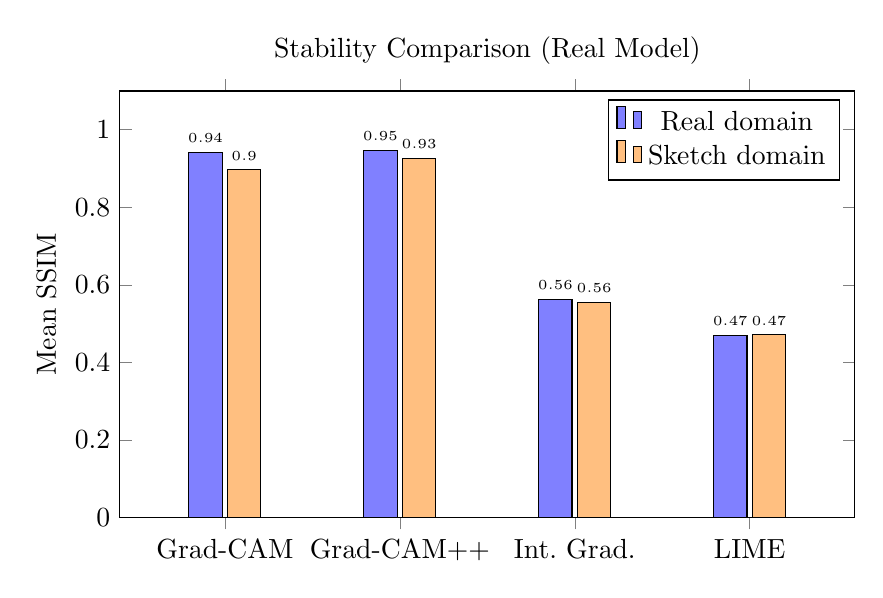
\begin{tikzpicture}
\begin{axis}[
    ybar,
    width=0.9\textwidth, height=7cm,
    ylabel={Mean SSIM},
    symbolic x coords={Grad-CAM, Grad-CAM++, Int.~Grad., LIME},
    xtick=data,
    legend style={at={(0.98,0.98)}, anchor=north east},
    ymin=0, ymax=1.1,
    bar width=12pt,
    title={Stability Comparison (Real Model)},
    enlarge x limits=0.2,
    nodes near coords,
    nodes near coords align={vertical},
    every node near coord/.append style={font=\tiny},
]
\addplot[fill=blue!50] coordinates {
    (Grad-CAM, 0.9418) (Grad-CAM++, 0.9458)
    (Int.~Grad., 0.5629) (LIME, 0.4706)
};
\addlegendentry{Real domain}
\addplot[fill=orange!50] coordinates {
    (Grad-CAM, 0.8964) (Grad-CAM++, 0.9269)
    (Int.~Grad., 0.5551) (LIME, 0.4710)
};
\addlegendentry{Sketch domain}
\end{axis}
\end{tikzpicture}
\caption{Stability (SSIM) comparison across methods for the real model.
CAM-based methods are substantially more stable than pixel-level methods.}
\label{fig:stability_real}
\end{figure}

\begin{figure}[H]
\centering
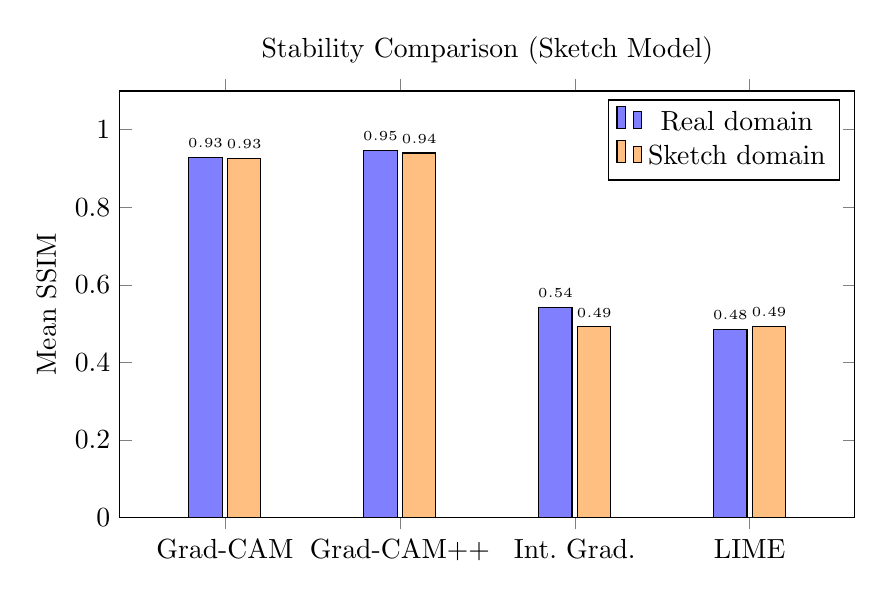
\begin{tikzpicture}
\begin{axis}[
    ybar,
    width=0.9\textwidth, height=7cm,
    ylabel={Mean SSIM},
    symbolic x coords={Grad-CAM, Grad-CAM++, Int.~Grad., LIME},
    xtick=data,
    legend style={at={(0.98,0.98)}, anchor=north east},
    ymin=0, ymax=1.1,
    bar width=12pt,
    title={Stability Comparison (Sketch Model)},
    enlarge x limits=0.2,
    nodes near coords,
    nodes near coords align={vertical},
    every node near coord/.append style={font=\tiny},
]
\addplot[fill=blue!50] coordinates {
    (Grad-CAM, 0.9280) (Grad-CAM++, 0.9464)
    (Int.~Grad., 0.5418) (LIME, 0.4847)
};
\addlegendentry{Real domain}
\addplot[fill=orange!50] coordinates {
    (Grad-CAM, 0.9264) (Grad-CAM++, 0.9401)
    (Int.~Grad., 0.4917) (LIME, 0.4929)
};
\addlegendentry{Sketch domain}
\end{axis}
\end{tikzpicture}
\caption{Stability (SSIM) comparison across methods for the sketch model.}
\label{fig:stability_sketch}
\end{figure}

\textbf{Key findings:}
\begin{itemize}[leftmargin=*]
    \item \textbf{Grad-CAM++ is the most stable method} across both models and
          domains (SSIM $\geq 0.92$).  Its higher-order gradient weighting
          provides robustness to small input perturbations.
    \item \textbf{Grad-CAM} is nearly as stable (SSIM $\approx 0.90$--$0.94$),
          with slightly lower scores on sketch images.
    \item \textbf{Integrated Gradients} shows moderate stability (SSIM
          $\approx 0.49$--$0.56$) with high variance.  Its pixel-level
          sensitivity makes it responsive to small noise.
    \item \textbf{LIME} is the least stable (SSIM $\approx 0.47$--$0.48$),
          reflecting its stochastic nature and sensitivity to superpixel
          boundaries.
    \item The stability gap between CAM-based and pixel-level methods is
          expected: the $7 \times 7$ spatial resolution of CAM methods acts as
          a natural low-pass filter that smooths out perturbation effects.
\end{itemize}

\subsection{Cross-Model Stability Comparison}

\begin{figure}[H]
\centering
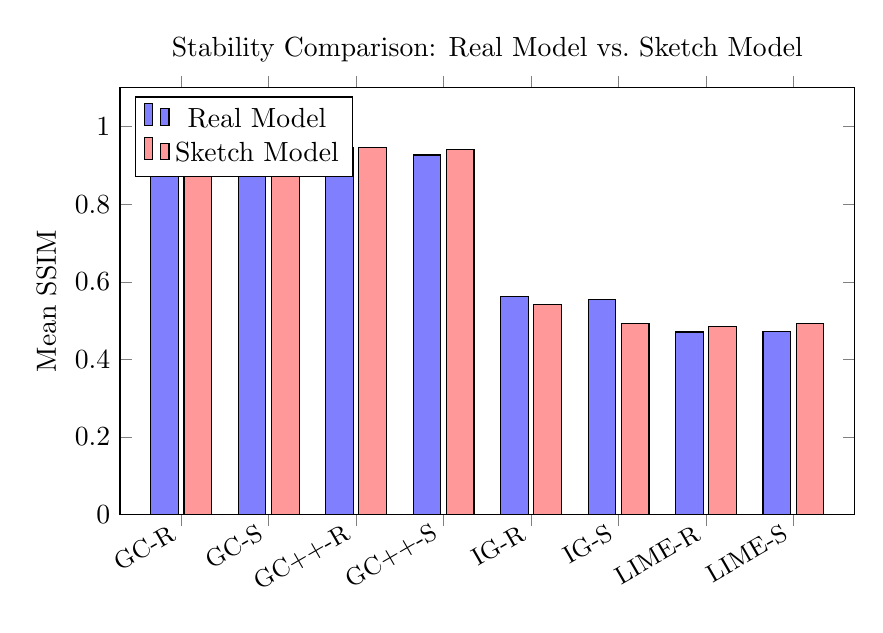
\begin{tikzpicture}
\begin{axis}[
    ybar,
    width=0.9\textwidth, height=7cm,
    ylabel={Mean SSIM},
    symbolic x coords={GC-R, GC-S, GC++-R, GC++-S, IG-R, IG-S, LIME-R, LIME-S},
    xtick=data,
    x tick label style={rotate=30, anchor=east, font=\small},
    legend style={at={(0.02,0.98)}, anchor=north west},
    ymin=0, ymax=1.1,
    bar width=10pt,
    title={Stability Comparison: Real Model vs.\ Sketch Model},
    enlarge x limits=0.1,
]
\addplot[fill=blue!50] coordinates {
    (GC-R, 0.9418) (GC-S, 0.8964) (GC++-R, 0.9458) (GC++-S, 0.9269)
    (IG-R, 0.5629) (IG-S, 0.5551) (LIME-R, 0.4706) (LIME-S, 0.4710)
};
\addlegendentry{Real Model}
\addplot[fill=red!40] coordinates {
    (GC-R, 0.9280) (GC-S, 0.9264) (GC++-R, 0.9464) (GC++-S, 0.9401)
    (IG-R, 0.5418) (IG-S, 0.4917) (LIME-R, 0.4847) (LIME-S, 0.4929)
};
\addlegendentry{Sketch Model}
\end{axis}
\end{tikzpicture}
\caption{Side-by-side stability comparison.  GC = Grad-CAM,
GC++ = Grad-CAM++, IG = Integrated Gradients.  R/S = real/sketch domain.
The sketch model shows more consistent stability across domains (GC-R
$\approx$ GC-S), while the real model's stability drops on sketch images.}
\label{fig:stability_comparison}
\end{figure}


% ── Faithfulness ──────────────────────────────────────────────────────────────
\subsection{Faithfulness Analysis}
\label{sec:faithfulness}

\textbf{Question:} Do the attribution maps actually identify the pixels that
the model relies on for its predictions?

Faithfulness is measured using two complementary metrics:
\begin{itemize}[leftmargin=*]
    \item \textbf{Deletion:} Pixels are removed in order of decreasing
          attribution score.  A faithful explanation causes a rapid confidence
          drop, yielding a \emph{high} deletion AUC (area under the confidence
          curve).
    \item \textbf{Insertion:} Pixels are revealed in order of decreasing
          attribution score onto a blank canvas.  A faithful explanation causes
          confidence to rise quickly, yielding a \emph{high} insertion AUC.
\end{itemize}

\begin{table}[H]
\centering
\caption{Faithfulness scores (Deletion AUC) for both models.  Higher values
indicate more faithful explanations.  Best values per model are \textbf{bolded}.}
\label{tab:deletion}
\begin{tabular}{llcccc}
\toprule
& & \multicolumn{2}{c}{\textbf{Real Model}} & \multicolumn{2}{c}{\textbf{Sketch Model}} \\
\cmidrule(lr){3-4} \cmidrule(lr){5-6}
\textbf{Method} & \textbf{Domain} & \textbf{Mean AUC} & \textbf{Std}
& \textbf{Mean AUC} & \textbf{Std} \\
\midrule
Grad-CAM   & real   & 0.2943 & 0.1904 & 0.1817 & 0.1643 \\
Grad-CAM   & sketch & 0.1069 & 0.1252 & 0.1696 & 0.1587 \\
Grad-CAM++ & real   & \textbf{0.3232} & 0.2021 & \textbf{0.2049} & 0.1776 \\
Grad-CAM++ & sketch & 0.1250 & 0.1384 & 0.1939 & 0.1716 \\
Int.~Grad. & real   & 0.2772 & 0.2042 & 0.1771 & 0.1968 \\
Int.~Grad. & sketch & 0.1247 & 0.1590 & 0.1722 & 0.1926 \\
LIME       & real   & 0.1524 & 0.1587 & 0.0706 & 0.0975 \\
LIME       & sketch & 0.0538 & 0.0895 & 0.0670 & 0.0933 \\
\bottomrule
\end{tabular}
\end{table}

\begin{table}[H]
\centering
\caption{Faithfulness scores (Insertion AUC) for both models.  Higher values
indicate more faithful explanations.  Best values per model are \textbf{bolded}.}
\label{tab:insertion}
\begin{tabular}{llcccc}
\toprule
& & \multicolumn{2}{c}{\textbf{Real Model}} & \multicolumn{2}{c}{\textbf{Sketch Model}} \\
\cmidrule(lr){3-4} \cmidrule(lr){5-6}
\textbf{Method} & \textbf{Domain} & \textbf{Mean AUC} & \textbf{Std}
& \textbf{Mean AUC} & \textbf{Std} \\
\midrule
Grad-CAM   & real   & 0.5475 & 0.1338 & 0.4727 & 0.1756 \\
Grad-CAM   & sketch & 0.3794 & 0.1743 & 0.4917 & 0.1700 \\
Grad-CAM++ & real   & 0.5370 & 0.1440 & 0.4531 & 0.1885 \\
Grad-CAM++ & sketch & 0.3446 & 0.1885 & 0.4700 & 0.1873 \\
Int.~Grad. & real   & 0.3519 & 0.1882 & 0.3209 & 0.2119 \\
Int.~Grad. & sketch & 0.2064 & 0.1767 & 0.2721 & 0.1924 \\
LIME       & real   & \textbf{0.6088} & 0.1054 & 0.5500 & 0.1581 \\
LIME       & sketch & 0.5013 & 0.1654 & \textbf{0.5707} & 0.1535 \\
\bottomrule
\end{tabular}
\end{table}

\begin{figure}[H]
\centering
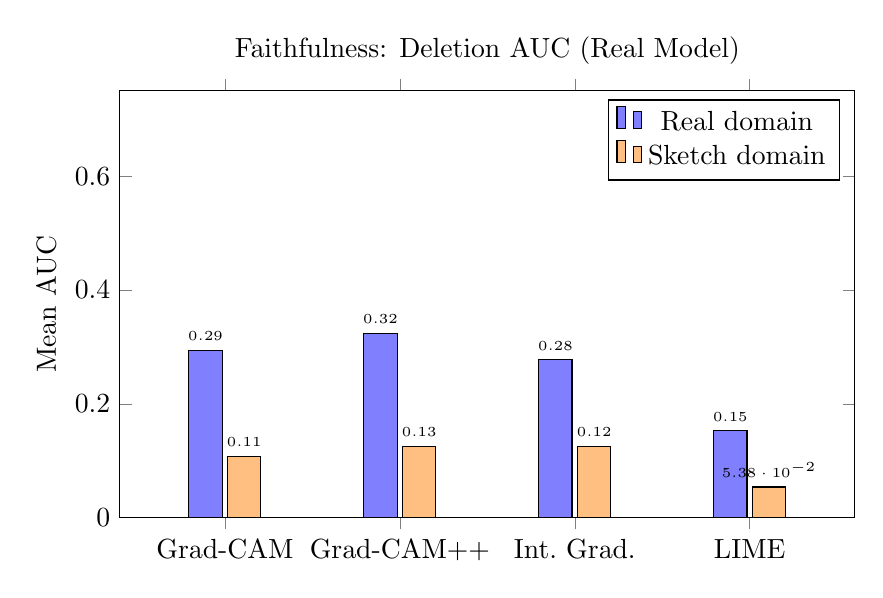
\begin{tikzpicture}
\begin{axis}[
    ybar,
    width=0.9\textwidth, height=7cm,
    ylabel={Mean AUC},
    symbolic x coords={Grad-CAM, Grad-CAM++, Int.~Grad., LIME},
    xtick=data,
    legend style={at={(0.98,0.98)}, anchor=north east},
    ymin=0, ymax=0.75,
    bar width=12pt,
    title={Faithfulness: Deletion AUC (Real Model)},
    enlarge x limits=0.2,
    nodes near coords,
    nodes near coords align={vertical},
    every node near coord/.append style={font=\tiny},
]
\addplot[fill=blue!50] coordinates {
    (Grad-CAM, 0.2943) (Grad-CAM++, 0.3232)
    (Int.~Grad., 0.2772) (LIME, 0.1524)
};
\addlegendentry{Real domain}
\addplot[fill=orange!50] coordinates {
    (Grad-CAM, 0.1069) (Grad-CAM++, 0.1250)
    (Int.~Grad., 0.1247) (LIME, 0.0538)
};
\addlegendentry{Sketch domain}
\end{axis}
\end{tikzpicture}
\caption{Deletion AUC for the real model.  Grad-CAM++ achieves the highest
deletion score, indicating its attribution maps best identify the model's
relied-upon features.  All methods show substantial drops on the sketch domain.}
\label{fig:deletion_real}
\end{figure}

\begin{figure}[H]
\centering
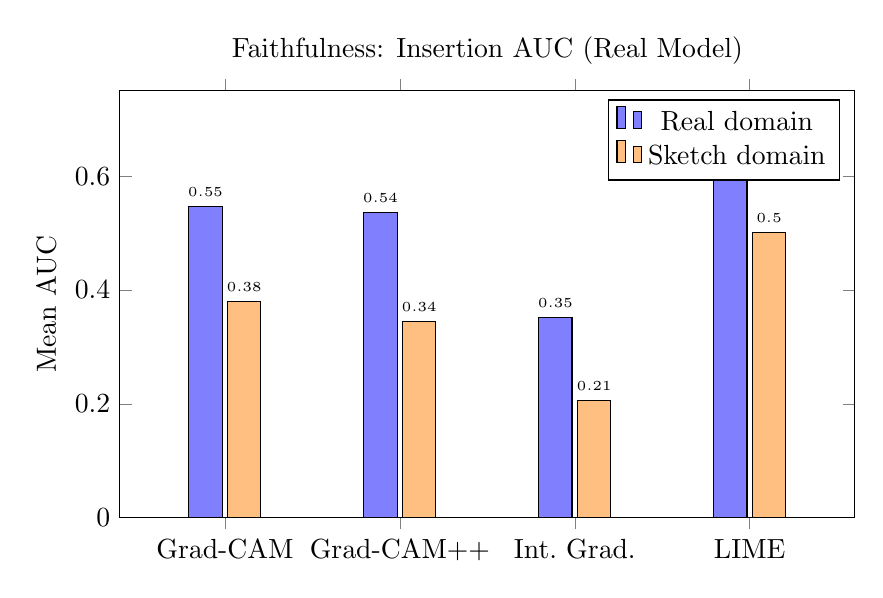
\begin{tikzpicture}
\begin{axis}[
    ybar,
    width=0.9\textwidth, height=7cm,
    ylabel={Mean AUC},
    symbolic x coords={Grad-CAM, Grad-CAM++, Int.~Grad., LIME},
    xtick=data,
    legend style={at={(0.98,0.98)}, anchor=north east},
    ymin=0, ymax=0.75,
    bar width=12pt,
    title={Faithfulness: Insertion AUC (Real Model)},
    enlarge x limits=0.2,
    nodes near coords,
    nodes near coords align={vertical},
    every node near coord/.append style={font=\tiny},
]
\addplot[fill=blue!50] coordinates {
    (Grad-CAM, 0.5475) (Grad-CAM++, 0.5370)
    (Int.~Grad., 0.3519) (LIME, 0.6088)
};
\addlegendentry{Real domain}
\addplot[fill=orange!50] coordinates {
    (Grad-CAM, 0.3794) (Grad-CAM++, 0.3446)
    (Int.~Grad., 0.2064) (LIME, 0.5013)
};
\addlegendentry{Sketch domain}
\end{axis}
\end{tikzpicture}
\caption{Insertion AUC for the real model.  LIME achieves the highest insertion
score, indicating its superpixel-based explanations most efficiently recover
model confidence.}
\label{fig:insertion_real}
\end{figure}

\begin{figure}[H]
\centering
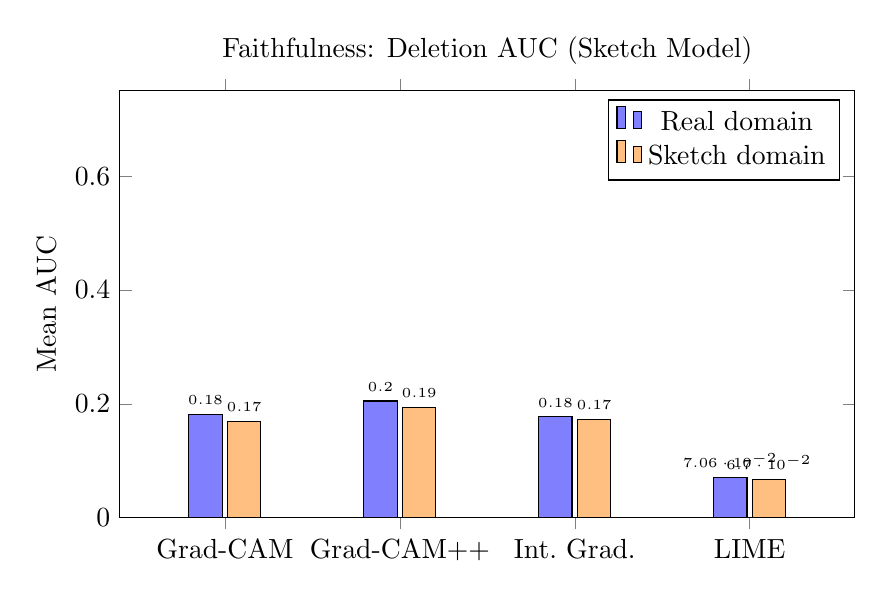
\begin{tikzpicture}
\begin{axis}[
    ybar,
    width=0.9\textwidth, height=7cm,
    ylabel={Mean AUC},
    symbolic x coords={Grad-CAM, Grad-CAM++, Int.~Grad., LIME},
    xtick=data,
    legend style={at={(0.98,0.98)}, anchor=north east},
    ymin=0, ymax=0.75,
    bar width=12pt,
    title={Faithfulness: Deletion AUC (Sketch Model)},
    enlarge x limits=0.2,
    nodes near coords,
    nodes near coords align={vertical},
    every node near coord/.append style={font=\tiny},
]
\addplot[fill=blue!50] coordinates {
    (Grad-CAM, 0.1817) (Grad-CAM++, 0.2049)
    (Int.~Grad., 0.1771) (LIME, 0.0706)
};
\addlegendentry{Real domain}
\addplot[fill=orange!50] coordinates {
    (Grad-CAM, 0.1696) (Grad-CAM++, 0.1939)
    (Int.~Grad., 0.1722) (LIME, 0.0670)
};
\addlegendentry{Sketch domain}
\end{axis}
\end{tikzpicture}
\caption{Deletion AUC for the sketch model.  Unlike the real model, the sketch
model shows similar faithfulness across both domains, reflecting its more
domain-invariant representations.}
\label{fig:deletion_sketch}
\end{figure}

\begin{figure}[H]
\centering
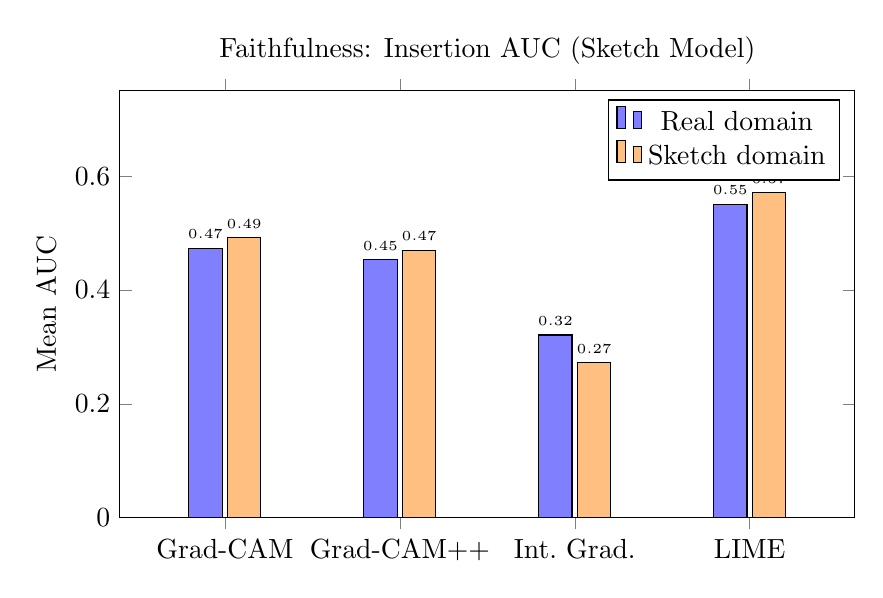
\begin{tikzpicture}
\begin{axis}[
    ybar,
    width=0.9\textwidth, height=7cm,
    ylabel={Mean AUC},
    symbolic x coords={Grad-CAM, Grad-CAM++, Int.~Grad., LIME},
    xtick=data,
    legend style={at={(0.98,0.98)}, anchor=north east},
    ymin=0, ymax=0.75,
    bar width=12pt,
    title={Faithfulness: Insertion AUC (Sketch Model)},
    enlarge x limits=0.2,
    nodes near coords,
    nodes near coords align={vertical},
    every node near coord/.append style={font=\tiny},
]
\addplot[fill=blue!50] coordinates {
    (Grad-CAM, 0.4727) (Grad-CAM++, 0.4531)
    (Int.~Grad., 0.3209) (LIME, 0.5500)
};
\addlegendentry{Real domain}
\addplot[fill=orange!50] coordinates {
    (Grad-CAM, 0.4917) (Grad-CAM++, 0.4700)
    (Int.~Grad., 0.2721) (LIME, 0.5707)
};
\addlegendentry{Sketch domain}
\end{axis}
\end{tikzpicture}
\caption{Insertion AUC for the sketch model.  LIME again leads on insertion,
and the sketch model's scores are remarkably balanced across domains.}
\label{fig:insertion_sketch}
\end{figure}

\textbf{Key findings:}
\begin{itemize}[leftmargin=*]
    \item \textbf{LIME is the most faithful by insertion AUC} across both models
          (0.61 real model / 0.57 sketch model on in-domain data).  Its
          superpixel-based approach effectively isolates the regions the model
          depends on, allowing rapid confidence recovery.
    \item \textbf{Grad-CAM++ leads on deletion AUC} (0.32 real model / 0.20
          sketch model), indicating its attributions best pinpoint the features
          whose removal most disrupts predictions.
    \item \textbf{Integrated Gradients underperforms on faithfulness} despite
          its pixel-level precision.  Its distributed attributions across many
          pixels make it harder to isolate critical features through sequential
          deletion/insertion.
    \item \textbf{Domain shift reduces faithfulness for the real model:}
          Deletion AUC drops from 0.29--0.32 (real domain) to 0.05--0.13
          (sketch domain), indicating the real model's explanations become less
          meaningful on out-of-domain data.
    \item \textbf{The sketch model shows balanced faithfulness:} Unlike the
          real model, the sketch model's deletion and insertion scores are
          similar across real and sketch domains (e.g., LIME insertion: 0.55
          vs.\ 0.57), confirming that shape-based representations produce
          more domain-invariant explanations.
\end{itemize}


% ── Cross-Domain Consistency ─────────────────────────────────────────────────
\subsection{Cross-Domain Consistency Analysis}
\label{sec:cross_domain}

\textbf{Question:} When the same class is viewed in different visual styles
(real vs.\ sketch), do the attribution maps highlight similar spatial regions?

For each class, we compute the average attribution map (prototype) over all
real images and all sketch images, then measure the \textbf{cosine similarity}
between these prototypes.  High similarity means the model uses consistent
features regardless of visual style.

\begin{table}[H]
\centering
\caption{Cross-domain consistency (mean cosine similarity across 81 classes).
Higher values indicate more consistent attributions across domains.
Best values per model are \textbf{bolded}.}
\label{tab:cross_domain}
\begin{tabular}{lcccc}
\toprule
& \multicolumn{2}{c}{\textbf{Real Model}} & \multicolumn{2}{c}{\textbf{Sketch Model}} \\
\cmidrule(lr){2-3} \cmidrule(lr){4-5}
\textbf{Method} & \textbf{Mean Cos.\ Sim.} & \textbf{Std}
& \textbf{Mean Cos.\ Sim.} & \textbf{Std} \\
\midrule
Grad-CAM           & 0.9526 & 0.0353 & 0.9491 & 0.0387 \\
Grad-CAM++         & \textbf{0.9626} & 0.0283 & \textbf{0.9608} & 0.0331 \\
Int.~Gradients     & 0.8418 & 0.0330 & 0.8953 & 0.0235 \\
LIME               & 0.8712 & 0.0423 & 0.8798 & 0.0411 \\
\bottomrule
\end{tabular}
\end{table}

\begin{figure}[H]
\centering
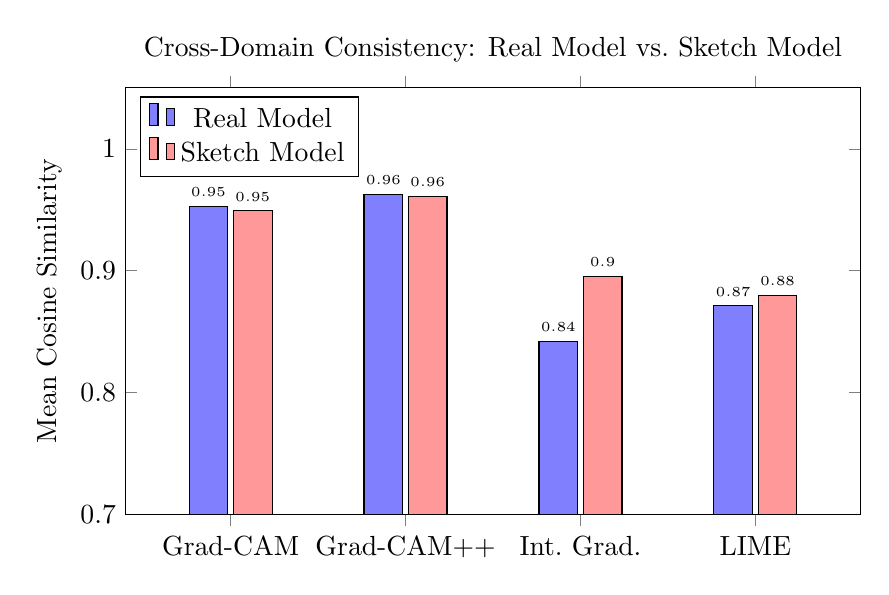
\begin{tikzpicture}
\begin{axis}[
    ybar,
    width=0.9\textwidth, height=7cm,
    ylabel={Mean Cosine Similarity},
    symbolic x coords={Grad-CAM, Grad-CAM++, Int.~Grad., LIME},
    xtick=data,
    legend style={at={(0.02,0.98)}, anchor=north west},
    ymin=0.7, ymax=1.05,
    bar width=14pt,
    title={Cross-Domain Consistency: Real Model vs.\ Sketch Model},
    enlarge x limits=0.2,
    nodes near coords,
    nodes near coords align={vertical},
    every node near coord/.append style={font=\tiny},
]
\addplot[fill=blue!50] coordinates {
    (Grad-CAM, 0.9526) (Grad-CAM++, 0.9626)
    (Int.~Grad., 0.8418) (LIME, 0.8712)
};
\addlegendentry{Real Model}
\addplot[fill=red!40] coordinates {
    (Grad-CAM, 0.9491) (Grad-CAM++, 0.9608)
    (Int.~Grad., 0.8953) (LIME, 0.8798)
};
\addlegendentry{Sketch Model}
\end{axis}
\end{tikzpicture}
\caption{Cross-domain consistency comparison.  CAM-based methods achieve
$>$0.95 cosine similarity, indicating very consistent spatial attention across
domains.  The sketch model's Integrated Gradients consistency (0.895) is notably
higher than the real model's (0.842), consistent with the shape bias hypothesis.}
\label{fig:cross_domain_bar}
\end{figure}

\textbf{Key findings:}
\begin{itemize}[leftmargin=*]
    \item \textbf{Grad-CAM++ achieves the highest cross-domain consistency}
          ($\geq 0.96$) for both models.  Its coarse spatial resolution
          naturally produces similar heatmaps regardless of visual style.
    \item \textbf{Grad-CAM is nearly as consistent} ($\approx 0.95$),
          confirming that CAM-based methods are robust to domain shift in
          their spatial attention patterns.
    \item \textbf{Integrated Gradients shows the largest model gap:} The
          sketch model (0.895) is substantially more consistent than the real
          model (0.842).  This indicates the sketch model's pixel-level
          attributions are more domain-invariant it attends to the same
          structural features (edges, contours) in both real and sketch images.
    \item \textbf{LIME} achieves moderate consistency ($\approx 0.87$--$0.88$),
          limited by its stochastic superpixel segmentation.
    \item The overall high consistency ($>$0.84 for all methods) suggests that
          despite performance degradation under domain shift, the models still
          attend to broadly similar spatial regions.
\end{itemize}


% ── Representation Analysis ──────────────────────────────────────────────────
\subsection{Representation Analysis}
\label{sec:representations}

\textbf{Question:} How does the model organise real and sketch images in its
learned feature space?

We extract penultimate-layer features (2048-dimensional) for all test images
from both domains and project them into 2D using t-SNE and UMAP.  Two
colourings reveal different aspects: \emph{by class} (do semantically similar
images cluster together?) and \emph{by domain} (does the model separate or
mix the two visual styles?).

\begin{figure}[H]
\centering
\begin{subfigure}[b]{0.48\textwidth}
    
\includegraphics[width=\textwidth]{output/xai/real_model/representations/tsne_by_class.png}
    \caption{t-SNE coloured by class}
\end{subfigure}
\hfill
\begin{subfigure}[b]{0.48\textwidth}
    
\includegraphics[width=\textwidth]{output/xai/real_model/representations/tsne_by_domain.png}
    \caption{t-SNE coloured by domain}
\end{subfigure}

\vspace{0.3cm}

\begin{subfigure}[b]{0.48\textwidth}
    
\includegraphics[width=\textwidth]{output/xai/real_model/representations/umap_by_class.png}
    \caption{UMAP coloured by class}
\end{subfigure}
\hfill
\begin{subfigure}[b]{0.48\textwidth}
    
\includegraphics[width=\textwidth]{output/xai/real_model/representations/umap_by_domain.png}
    \caption{UMAP coloured by domain}
\end{subfigure}
\caption{\textbf{Real model --- feature space visualisations.}
The t-SNE by-class plot (a) shows well-separated class clusters for real images,
but sketch images from the same class often fall outside these clusters.
The by-domain plot (b) reveals a clear separation between real (blue) and sketch
(orange) points, indicating the real model encodes domain-specific features.
UMAP (c, d) confirms this pattern with tighter, more separated clusters.}
\label{fig:repr_real}
\end{figure}

\begin{figure}[H]
\centering
\begin{subfigure}[b]{0.48\textwidth}
    
\includegraphics[width=\textwidth]{output/xai/sketch_model/representations/tsne_by_class.png}
    \caption{t-SNE coloured by class}
\end{subfigure}
\hfill
\begin{subfigure}[b]{0.48\textwidth}
    
\includegraphics[width=\textwidth]{output/xai/sketch_model/representations/tsne_by_domain.png}
    \caption{t-SNE coloured by domain}
\end{subfigure}

\vspace{0.3cm}

\begin{subfigure}[b]{0.48\textwidth}
    
\includegraphics[width=\textwidth]{output/xai/sketch_model/representations/umap_by_class.png}
    \caption{UMAP coloured by class}
\end{subfigure}
\hfill
\begin{subfigure}[b]{0.48\textwidth}
    
\includegraphics[width=\textwidth]{output/xai/sketch_model/representations/umap_by_domain.png}
    \caption{UMAP coloured by domain}
\end{subfigure}
\caption{\textbf{Sketch model --- feature space visualisations.}
The by-domain plots (b, d) show substantially more overlap between real and
sketch points compared to the real model (Figure~\ref{fig:repr_real}).  This
confirms that the sketch model learns \emph{domain-invariant} representations
--- real and sketch images of the same class are mapped to similar locations
in feature space, explaining the sketch model's superior cross-domain transfer.}
\label{fig:repr_sketch}
\end{figure}

\textbf{Key findings:}
\begin{itemize}[leftmargin=*]
    \item \textbf{The real model separates domains:} In its feature space, real
          and sketch images form distinct clusters even for the same class.
          This domain separation explains the 37-point accuracy drop when
          transferring to sketches.
    \item \textbf{The sketch model mixes domains:} Real and sketch images
          are more interleaved in the sketch model's feature space, with
          same-class images from both domains occupying overlapping regions.
          This domain-invariant organisation explains the sketch model's
          superior transfer performance.
    \item \textbf{Class structure is preserved in both models:} Despite
          differences in domain separation, both models produce coherent
          class clusters, confirming that the 81-class classification task
          has been successfully learned.
    \item These visualisations provide direct evidence for the \emph{shape
          bias hypothesis}: the sketch model's shape-based features create a
          domain-agnostic feature space, while the real model's texture-based
          features encode domain identity alongside class identity.
\end{itemize}


% ══════════════════════════════════════════════════════════════════════════════
\section{Discussion}
\label{sec:discussion}

\subsection{Domain Transfer Asymmetry}

The most striking finding is the \textbf{asymmetric transfer} between domains.
The sketch$\to$real transfer (83.02\%) substantially outperforms real$\to$sketch
(56.17\%).  This result aligns with the \emph{texture bias} hypothesis: CNNs
trained on photographs tend to rely on texture cues (colour gradients, surface
patterns) that are absent in line drawings.  Conversely, sketch training forces
the model to rely on \emph{shape-based} features (edges, contours, spatial
relationships) that are present in both domains.

\begin{figure}[H]
\centering
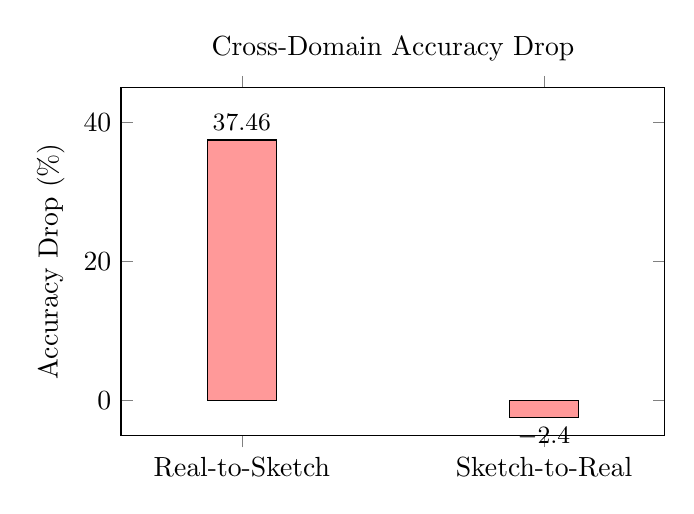
\begin{tikzpicture}
\begin{axis}[
    ybar,
    width=0.7\textwidth, height=6cm,
    ylabel={Accuracy Drop (\%)},
    symbolic x coords={Real-to-Sketch, Sketch-to-Real},
    xtick=data,
    ymin=-5, ymax=45,
    bar width=25pt,
    title={Cross-Domain Accuracy Drop},
    nodes near coords,
    nodes near coords align={vertical},
    every node near coord/.append style={font=\small},
    enlarge x limits=0.4,
]
\addplot[fill=red!40] coordinates {
    (Real-to-Sketch, 37.46)
    (Sketch-to-Real, -2.40)
};
\end{axis}
\end{tikzpicture}
\caption{Cross-domain accuracy drop relative to in-domain performance.  The
real model loses 37.46\% when transferred to sketch, while the sketch model
actually \emph{gains} 2.40\% when transferred to real images.}
\label{fig:domain_drop}
\end{figure}

\subsection{Stability vs.\ Granularity Trade-off}

There is a clear trade-off between explanation stability and spatial
granularity:

\begin{itemize}[leftmargin=*]
    \item CAM-based methods (Grad-CAM, Grad-CAM++) operate at $7 \times 7$
          resolution, which acts as a natural low-pass filter.  This makes them
          highly stable (SSIM $> 0.90$) but unable to capture fine-grained
          details.
    \item Integrated Gradients operates at full $224 \times 224$ resolution,
          capturing pixel-level details but at the cost of perturbation
          sensitivity (SSIM $\approx 0.50$).
    \item LIME operates at superpixel resolution, with inherent stochasticity
          from its sampling-based approach.
\end{itemize}

\begin{figure}[H]
\centering
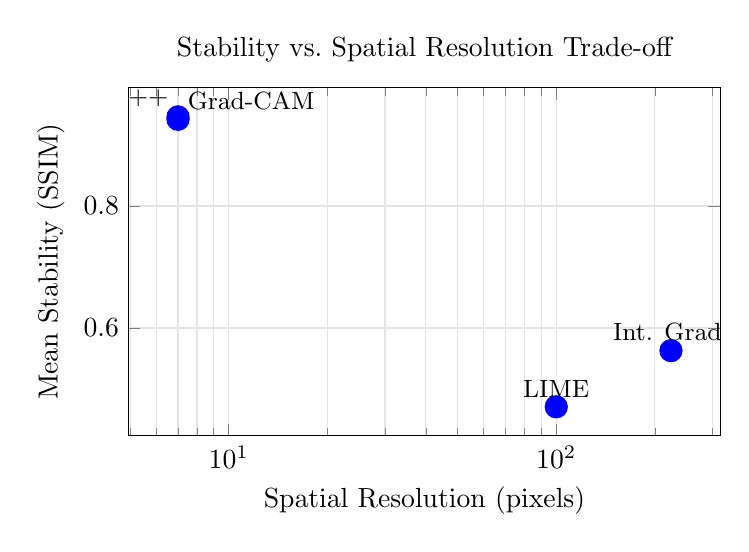
\begin{tikzpicture}
\begin{axis}[
    width=0.75\textwidth, height=6cm,
    xlabel={Spatial Resolution (pixels)},
    ylabel={Mean Stability (SSIM)},
    xmode=log,
    grid=both, grid style={gray!20},
    title={Stability vs.\ Spatial Resolution Trade-off},
]
\addplot[only marks, mark=*, mark size=4pt, blue] coordinates {
    (7, 0.942) (7, 0.946) (224, 0.563) (100, 0.471)
};
\node[above right, font=\small] at (axis cs:7,0.942) {Grad-CAM};
\node[above left, font=\small] at (axis cs:7,0.946) {Grad-CAM++};
\node[above, font=\small] at (axis cs:224,0.563) {Int. Grad.};
\node[above, font=\small] at (axis cs:100,0.471) {LIME};
\end{axis}
\end{tikzpicture}
\caption{The stability-granularity trade-off.  Methods with coarser spatial
resolution are more stable under perturbation.}
\label{fig:stability_tradeoff}
\end{figure}

\subsection{Explanation Quality Under Domain Shift}

Our cross-domain attribution comparisons (Figures~\ref{fig:attr_cross_bicycle},
\ref{fig:attr_banana_cross}, \ref{fig:attr_tiger_cross}) and the quantitative
faithfulness results (Section~\ref{sec:faithfulness}) confirm that
\textbf{domain shift degrades explanation quality}, not just classification
accuracy.  When the real model is applied to sketches:

\begin{itemize}[leftmargin=*]
    \item Attribution maps become more diffuse and less focused on the object.
    \item Faithfulness drops sharply: deletion AUC falls from 0.29--0.32 to
          0.05--0.13, indicating the explanations no longer identify the
          model's actual decision features.
    \item LIME and Integrated Gradients show more scattered attributions,
          suggesting the model is ``guessing'' rather than using learned
          features.
\end{itemize}

In contrast, the sketch model's attributions on real images remain relatively
focused, and its faithfulness scores are balanced across domains (e.g., LIME
insertion: 0.55 real vs.\ 0.57 sketch).  The representation analysis
(Section~\ref{sec:representations}) provides a mechanistic explanation: the
sketch model's feature space mixes domains, while the real model separates
them, directly explaining the asymmetric transfer and explanation degradation.

\subsection{Implications for Practitioner Choice}

Based on our analysis, we recommend:

\begin{itemize}[leftmargin=*]
    \item \textbf{For quick, reliable explanations:} Use Grad-CAM++ it
          offers the best stability while providing class-discriminative
          spatial highlighting.
    \item \textbf{For detailed pixel-level analysis:} Use Integrated Gradients
           despite lower stability, its axiomatic guarantees make it
          suitable for rigorous analysis.
    \item \textbf{For model-agnostic explanations:} Use LIME  when the
          model architecture is unknown, LIME is the only option, though
          users should be aware of its stochastic nature.
    \item \textbf{For cross-domain studies:} Consider training on sketches or
          shape-biased data to improve both classification transfer and
          explanation consistency.
\end{itemize}


% ══════════════════════════════════════════════════════════════════════════════
\section{Pipeline Overview}
\label{sec:pipeline}

The complete pipeline consists of four stages executed sequentially:

\begin{figure}[H]
\centering
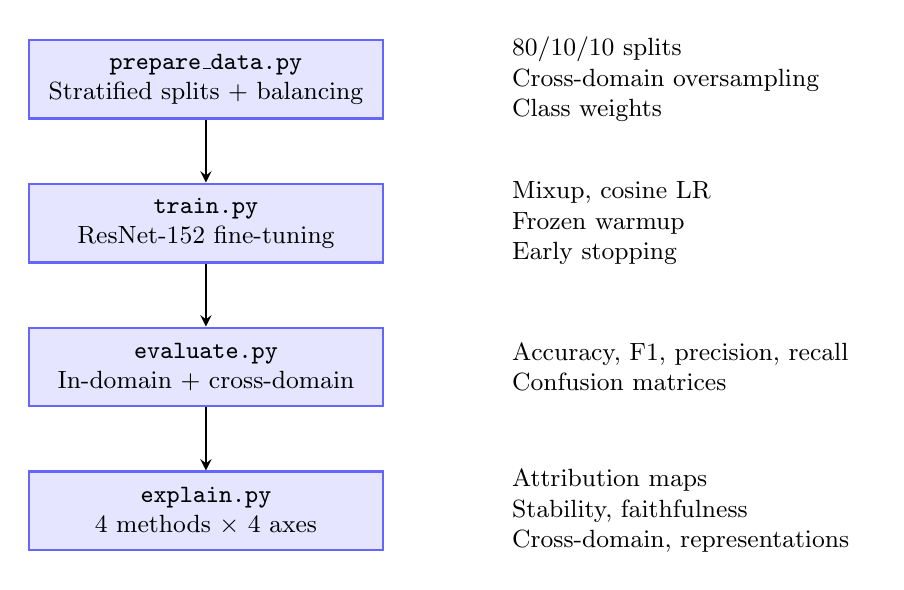
\begin{tikzpicture}[
    node distance=0.8cm,
    box/.style={rectangle, draw=blue!60, fill=blue!10, thick,
                minimum width=4.5cm, minimum height=1cm, align=center,
                font=\small},
    arrow/.style={->, >=stealth, thick},
]
\node[box] (prep) {\texttt{prepare\_data.py}\\Stratified splits + balancing};
\node[box, below=of prep] (train) {\texttt{train.py}\\ResNet-152 fine-tuning};
\node[box, below=of train] (eval) {\texttt{evaluate.py}\\In-domain + cross-domain};
\node[box, below=of eval] (xai) {\texttt{explain.py}\\4 methods $\times$ 4 axes};

\draw[arrow] (prep) -- (train);
\draw[arrow] (train) -- (eval);
\draw[arrow] (eval) -- (xai);

\node[right=1.5cm of prep, font=\small, text width=4.5cm]
    {80/10/10 splits\\Cross-domain oversampling\\Class weights};
\node[right=1.5cm of train, font=\small, text width=4.5cm]
    {Mixup, cosine LR\\Frozen warmup\\Early stopping};
\node[right=1.5cm of eval, font=\small, text width=4.5cm]
    {Accuracy, F1, precision, recall\\Confusion matrices};
\node[right=1.5cm of xai, font=\small, text width=4.5cm]
    {Attribution maps\\Stability, faithfulness\\Cross-domain, representations};
\end{tikzpicture}
\caption{Complete pipeline architecture.}
\label{fig:pipeline}
\end{figure}


% ══════════════════════════════════════════════════════════════════════════════
\section{Conclusion}
\label{sec:conclusion}

This study presents a systematic evaluation of four XAI attribution methods
applied to ResNet-152 classifiers trained on two visual domains from DomainNet.
Our key findings are:

\begin{enumerate}[leftmargin=*]
    \item \textbf{Sketch-trained models generalise better:}  The sketch model
          transfers to real images (83.02\%) far more effectively than the real
          model transfers to sketches (56.17\%), confirming that shape-based
          representations are more domain-invariant than texture-based ones.

    \item \textbf{Domain shift degrades explanations:}  Not only does
          classification accuracy drop under domain shift, but the quality of
          XAI explanations also deteriorates attributions become diffuse,
          unfocused, and less semantically meaningful.

    \item \textbf{CAM-based methods are most stable and consistent:}
          Grad-CAM++ achieves the highest stability (SSIM $\approx 0.94$) and
          cross-domain consistency (cosine similarity $\geq 0.96$) across both
          models, making it the most reliable choice for applications requiring
          consistent explanations.

    \item \textbf{LIME is the most faithful:}  Despite low stability, LIME
          achieves the highest insertion AUC ($\approx 0.57$--$0.61$),
          demonstrating that its superpixel-based explanations best capture
          the features the model actually relies on.

    \item \textbf{Granularity-stability trade-off:}  Pixel-level methods
          (Integrated Gradients, LIME) provide finer spatial detail but are
          significantly less stable under input perturbation (SSIM $\approx
          0.47$--$0.56$).

    \item \textbf{Domain-invariant representations explain transfer:}
          The sketch model's feature space intermixes real and sketch images
          (visible in t-SNE/UMAP), while the real model separates them 
          directly explaining the asymmetric transfer performance.

    \item \textbf{XAI evaluation must be multi-axis:}  No single method
          dominates across all evaluation criteria.  A comprehensive assessment
          requires measuring stability, faithfulness, cross-domain consistency,
          and representation structure jointly.
\end{enumerate}

\subsection{Future Work}

\begin{itemize}[leftmargin=*]
    \item Extend the study to additional DomainNet domains (clipart, painting,
          quickdraw) to test generality of the findings across more diverse
          visual styles.
    \item Investigate shape-biased training augmentations (stylisation,
          edge-detection preprocessing) to improve real$\to$sketch transfer.
    \item Apply more recent XAI methods (e.g., Attention Rollout, SHAP,
          Score-CAM) for broader comparison.
    \item Develop quantitative metrics for domain separation in feature space
          to complement the qualitative t-SNE/UMAP visualisations.
    \item Investigate whether fine-tuning with domain-adversarial training
          can reduce the real model's domain separation and improve both
          transfer accuracy and explanation consistency.
\end{itemize}


% ══════════════════════════════════════════════════════════════════════════════
\begin{thebibliography}{9}

\bibitem{domainnet}
X.~Peng, Q.~Bai, X.~Xia, Z.~Huang, K.~Saenko, and B.~Wang,
``Moment matching for multi-source domain adaptation,''
in \emph{Proc.\ IEEE/CVF ICCV}, 2019, pp.~1406--1415.

\bibitem{selvaraju2017gradcam}
R.~R. Selvaraju, M.~Cogswell, A.~Das, R.~Vedantam, D.~Parikh, and D.~Batra,
``Grad-CAM: Visual explanations from deep networks via gradient-based
localization,''
in \emph{Proc.\ IEEE ICCV}, 2017, pp.~618--626.

\bibitem{chattopadhay2018gradcampp}
A.~Chattopadhay, A.~Sarkar, P.~Howlader, and V.~N. Balasubramanian,
``Grad-CAM++: Generalized gradient-based visual explanations for deep
convolutional networks,''
in \emph{Proc.\ IEEE WACV}, 2018, pp.~839--847.

\bibitem{sundararajan2017ig}
M.~Sundararajan, A.~Taly, and Q.~Yan,
``Axiomatic attribution for deep networks,''
in \emph{Proc.\ ICML}, vol.~70, 2017, pp.~3319--3328.

\bibitem{ribeiro2016lime}
M.~T. Ribeiro, S.~Singh, and C.~Guestrin,
``{`Why should I trust you?'}: Explaining the predictions of any classifier,''
in \emph{Proc.\ ACM SIGKDD}, 2016, pp.~1135--1144.

\bibitem{he2016resnet}
K.~He, X.~Zhang, S.~Ren, and J.~Sun,
``Deep residual learning for image recognition,''
in \emph{Proc.\ IEEE CVPR}, 2016, pp.~770--778.

\bibitem{geirhos2019texture}
R.~Geirhos, P.~Rubisch, C.~Michaelis, M.~Bethge, F.~A. Wichmann, and
W.~Brendel,
``ImageNet-trained {CNN}s are biased towards texture; increasing shape bias
improves accuracy and robustness,''
in \emph{Proc.\ ICLR}, 2019.

\bibitem{zhang2018mixup}
H.~Zhang, M.~Cisse, Y.~N. Dauphin, and D.~Lopez-Paz,
``mixup: Beyond empirical risk minimization,''
in \emph{Proc.\ ICLR}, 2018.

\end{thebibliography}

% ══════════════════════════════════════════════════════════════════════════════
\appendix

\section{Hyperparameter Summary}
\label{app:hyperparams}

\begin{table}[H]
\centering
\caption{Complete hyperparameter configuration.}
\label{tab:hyperparams}
\begin{tabular}{llr}
\toprule
\textbf{Category} & \textbf{Parameter} & \textbf{Value} \\
\midrule
\multirow{3}{*}{Data}
    & Number of classes       & 81 \\
    & Train/val/test split    & 80/10/10 \\
    & Image size              & $224 \times 224$ \\
\midrule
\multirow{8}{*}{Training}
    & Backbone                & ResNet-152 \\
    & Pretrained weights      & ImageNet-1K V2 \\
    & Optimizer               & AdamW \\
    & Base learning rate      & $10^{-3}$ \\
    & Weight decay            & $5 \times 10^{-4}$ \\
    & Batch size              & 256 \\
    & Max epochs              & 100 \\
    & Early stopping patience & 10 \\
    & Warmup epochs           & 5 \\
    & Mixup $\alpha$          & 0.2 \\
    & Label smoothing         & 0.1 \\
    & Freeze epochs           & 5 \\
\midrule
\multirow{5}{*}{XAI}
    & Samples per class/domain & 20 \\
    & IG interpolation steps   & 100 \\
    & LIME perturbation samples & 3{,}000 \\
    & LIME superpixels          & 150 \\
    & Stability perturbations   & 5 \\
\bottomrule
\end{tabular}
\end{table}

\end{document}
